\documentclass[11pt,a4paper]{article}
\usepackage[utf8]{inputenc}
\usepackage[english]{babel}
\usepackage{amsmath}
\usepackage{amsfonts}
\usepackage{amssymb}
\usepackage{ragged2e}
\usepackage{graphicx}
\usepackage{float}
\usepackage{hyperref}
\usepackage{array}
\usepackage{subcaption}
\usepackage[bottom]{footmisc}

\usepackage[left=3cm,right=3cm,top=3cm,bottom=3cm]{geometry}
\begin{document}



\justifying

%%%%%%%%%%%%%%%%%%%%%%%%%%%%%%%%%%%%%%%%%%%%%%%%%%
%%%%%%%%%%%%%%%%%%% TITLE PAGE %%%%%%%%%%%%%%%%%%%
%%%%%%%%%%%%%%%%%%%%%%%%%%%%%%%%%%%%%%%%%%%%%%%%%%

\begin{titlepage}
\begin{center}
{{\Large{\textsc{Motorvehicle University of Emilia-Romagna}}}} \rule[0.1cm]{15.8cm}{0.1mm}
\rule[0.5cm]{15.8cm}{0.6mm}
Master Degree in Advanced Automotive Electronic Engineering

\end{center}

\vspace{15mm}
\begin{center}
{\LARGE{\bf MPC for Dynamic Obstacle Avoidance}}
\rule[0.1cm]{15.8cm}{0.1mm}
\begin{LARGE}

Technical report on the group project activity\\


\end{LARGE}
\vspace{5mm}
Course of Compliance Design of Automotive Systems
\end{center}

\begin{center}
 \begin{figure}[H]
          
\includegraphics[width=1\textwidth]{Figures/MUNER_logo.jpg}
          \end{figure}

 {\large\bf Group memebers:\\}
 {Gianvincenzo Daddabbo}\\
{Gaetano Gallo}\\
{Alberto Ruggeri}\\
{Martina Tedesco}\\
{Alessandro Toschi}\\



\vspace{4mm}
{\large\bf a.y. 2020-2021}
\end{center}
\end{titlepage}

%%%%%%%%%%%%%%%%%%%%%%%%%%%%
%%%%%%%%% Abstract %%%%%%%%%
%%%%%%%%%%%%%%%%%%%%%%%%%%%%

\begin{abstract}
Every year 1.25 million people die and as many as 50 million are injured in road
traffic accidents worldwide, according to United Nations statistics. Human error is involved in about 95\% of all road traffic accidents in the EU, and in 2017 alone, 25300 people died on the Union’s roads \cite{frisoni2016research}.  
Autonomous cars can improve road safety and through new technologies it is also possible to reduce traffic congestion and CO2 emissions.\\
The aim of this report is to present the steps that we have followed as a group in order to implement a system for dynamic obstacle avoidance using an adaptive Model Predictive Control. 
In the simulated environment, the vehicle model is expected to encounter and safely avoid the dynamic obstacles along its way. 
On the other hand, when an obstacle is not present ahead of the autonomous vehicle, it is expected to follow a predetermined path.

\end{abstract}

\newpage
\tableofcontents
\newpage
\listoffigures
\newpage
\listoftables
\newpage

\section{Introduction}
\label{sec:intro}
\begin{center}
\emph{``Every year 1.25 million people die and as many as 50 million are injured in road
traffic accidents worldwide, according to United Nations statistics. Human error is involved in about 95\% of all road traffic accidents in the EU, and in 2017 alone, 25300 people died on the Union’s roads." \cite{frisoni2016research}}\\
\end{center}
Autonomous cars can improve road safety and through new technologies it is also possible to reduce traffic congestion and CO2 emissions.
The task of avoiding obstacles is one of the key issues when it comes to the vehicular scenario and it is more difficult to perform it here than it is in static environments.
A vehicle with  an obstacles avoidance system is equipped with sensors that measure the distance between the car itself and the obstacle in the same lane. If an autonomous car encounters an obstacle, it is expected to move temporarily to another lane and move back to the original lane once it has driven past the obstacle.
The aim of this report is to present the steps that we have followed as a group in order to implement a system for dynamic obstacle avoidance using an adaptive Model Predictive Control. 
In particular, the report is structured as follows:
\begin{itemize}
    \item the introduction of this report focuses on the basics behind the concepts of Model Predictive Control and Model-Based Design and ends by introducing the software tools used in the project;
    \item starting from Section 2 up to Section 4 we go through the set of requirements of our project laid down by a hypothetical customer, the corresponding low level requirements and the associated validation methods, as well as introducing the system partitioning adopted during the development phase and the mathematical model behind our ego vehicle;
    \item in Section 5 and 6 we go through the various technologies available on the market related to the perception, route planning and control of autonomous vehicles explaining our assumptions regarding these topics. We then proceed explaining how we have imported real maps into our simulation environment and the constraints we have taken into account concerning throttle, steering angle and outputs;
    \item the sections from 7 to 12 are dedicated to the presentation of the actual controller setup and the tests performed in order to validate our controller against the path following task and obstacle avoidance tasks (both static and dynamic, both single and multiple);
   \item the report ends with some considerations on the project carried out and some ideas to further improve it.
\end{itemize}



\subsection{MPC: basic concepts}
In the simulated environment, the vehicle model is expected to encounter and safely avoid obstacles along its way. On the other hand, when an obstacle is not present ahead of the autonomous vehicle, it is expected to follow a predetermined path.
This type of control can be implemented using a Model Predictive Control (MPC).
An MPC is an advanced control method that works in discrete time and uses a model of the system to make predictions about the system’s future behavior. 
Figure \ref{fig:MPC_scheme} graphically shows the general concept behind a Model Predictive Control.
\begin{figure}[H]
    \centering
    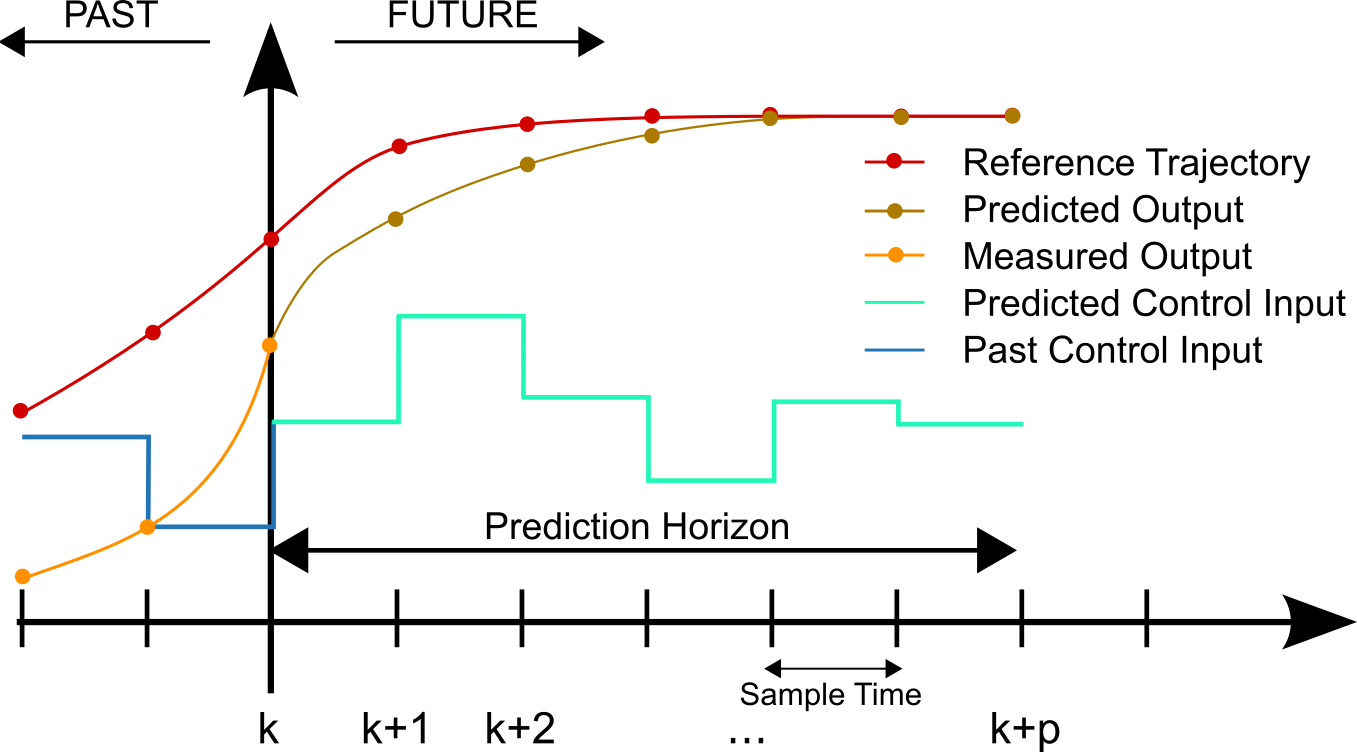
\includegraphics[width=0.9\textwidth]{Figures/MPC_scheme_basic.png}
    \caption{MPC algorithm scheme}
    \label{fig:MPC_scheme}
\end{figure}
The MPC solves an online optimization algorithm to find the optimal control action that drives the predicted output to the reference \cite{MPC_Def}. In other words, from a set of state values, and with respect to a model, it optimizes a problem around an objective and gives a sequence of control signals as outputs. The first set of control values are then used as inputs to the system plant, and after a short period, set as the \emph{system time step}, the new state values are measured and the process is repeated.
The overall objectives of the MPC are:
\begin{itemize}
 

\item prevent that input and output constraints are violated;
\item optimize some input variables, while other outputs are kept in specified ranges;
\item prevent the input variables from having excessive variations.
\end{itemize}
Figure \ref{fig:MPC_Block} shows a block diagram for a Model Predictive Control.
\begin{figure}[H]
    \centering
    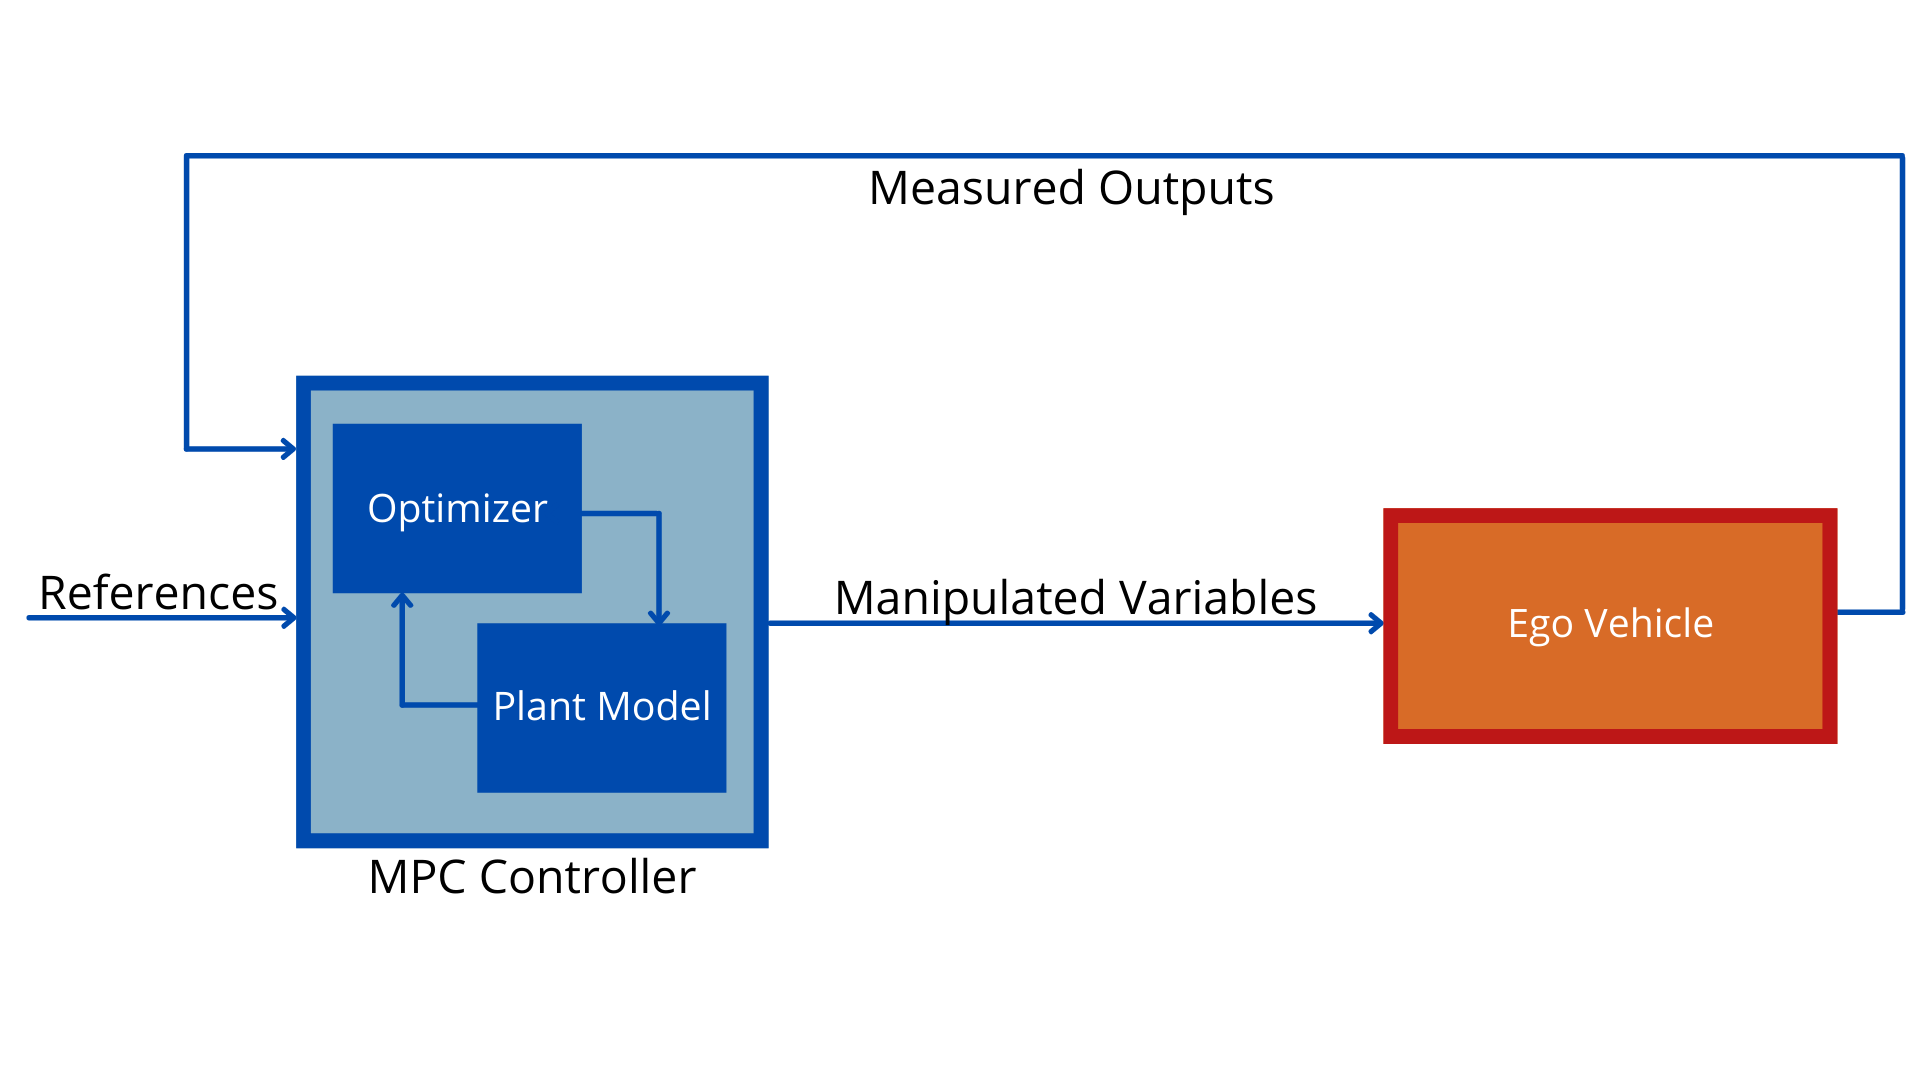
\includegraphics[width=1\textwidth]{Figures/mpcblock.png}
    \caption{MPC Block Diagram}
      \label{fig:MPC_Block}
\end{figure}
An MPC controller has two main functional blocks: the optimizer and the plant model.
The dynamic optimizer allows to find the optimal input that gives the minimum
value of the cost function taking into account all the constraints. Generally, a non linear model is used for the validation of the controller, while the plant model used for the MPC is a linearized version of the actual plant.\\
Our project is based on the use of an \emph{adaptive} MPC, which means that the plant state has to be measured again to be adopted as the linearization point for the next step of the predictive control. When the plant state is re-sampled, the whole process
computes again the calculations starting from the new current state.

\subsection{Model-Based Design}
When developing a project, especially concerning embedded systems, it is crucial to follow a process model which illustrates the high-level activities and their phasing during development.\\
As stated in \cite{FOWLER20151} \emph{``Process models provide high-level perspective that helps team members understand what activities to do and what progress  has been made on each of those development activities"}.\\
The development process of our system is based on the V-model shown in Figure \ref{fig:V_model}.
Starting from the general V-model we have tailored our own V-model in order to meet our needs; doing so we have managed to skip some unnecessary steps in the development process while still being compliant with the definition of the V-model itself.

\begin{figure}[H]
    \centering
    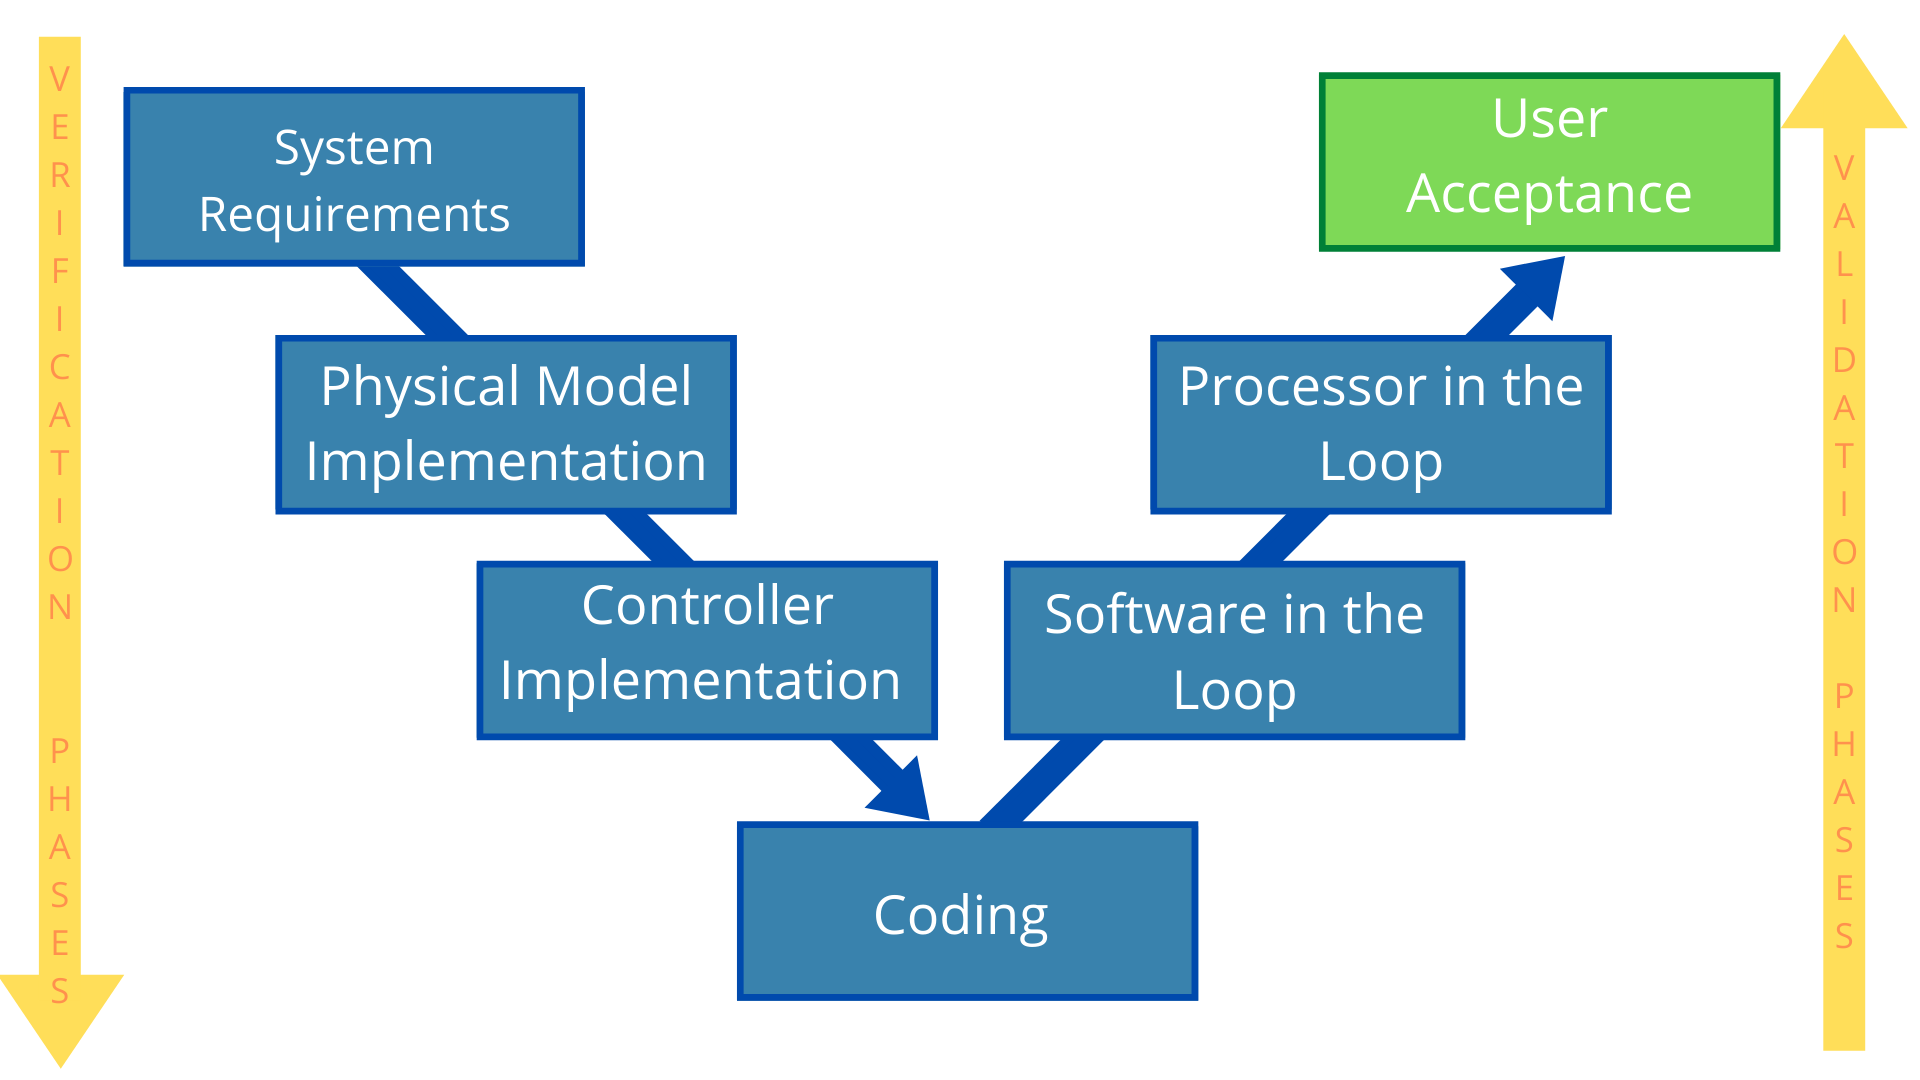
\includegraphics[width=1\textwidth]{Figures/V-MODEL.png}
    \caption{System Development V-model}
    
    \label{fig:V_model}
\end{figure}

As shown above the V-model is a representation of the system development process that highlights verification steps on one side and validation steps on the other of the ``V". The left side of the ``V" identifies the verification phase, containing the steps that lead to code generation while the right side identifies the validation phase which ends with the user acceptance.
Below a brief description of the steps that constitute our V-model:
\begin{itemize}
    \item \textbf{System requirements}: this is the first step of each project, it consists in gathering the requirements from the customer;
    \item \textbf{Physical model implementation}: this phase contains the system design of our vehicle in terms of sensors required and dynamic and kinematic model;
    \item \textbf{Controller implementation}: this phase represents the focus of our project, designing an adaptive MPC;
    \item \textbf{Coding}: exploiting some specific tools, we can automatically generate code for embedded deployment and create test benches for system verification, saving time and avoiding the introduction of manually coded errors;
    \item \textbf{Software-in-the-Loop}: once generated, the code is tested in a simulation environment;
    
    \item \textbf{Processor-in-the-Loop}: during this phase the code is uploaded on a demo board and than it is tested again;
    
    \item \textbf{User Acceptance}: in this phase the final product is tested in order to verify the compliance with the initial costumer requirements.
\end{itemize}

\subsection{Required tools}
The project is based on \href{https://www.mathworks.com/help/matlab/index.html?s_tid=srchtitle}{\underline{MATLAB}}, a proprietary multi-paradigm programming language and numeric computing environment developed by \textit{MathWorks}, and \href{https://www.mathworks.com/help/simulink/index.html?s_tid=CRUX_lftnav}{\underline{Simulink}}, a MATLAB-based block diagram environment for multi-domain simulation and Model-Based Design.\\
The software requirements for the project, including all the applications needed for the proper execution and test are listed below:
\begin{itemize}
    \item \textbf{MATLAB R2019a or newer};
    \begin{enumerate}
            \item \textbf{Curve Fitting Toolbox}: needed to make the reference map smoother;
            \item \textbf{Automated Driving Toolbox}: needed to import a reference map from real world data;
            \item \textbf{Model Predictive Control Toolbox}: needed to have all the useful resources to develop the MPC.
    \end{enumerate}
    \item \textbf{Simulink 9.3 or higher};
    \begin{enumerate}
            \item \textbf{Simulink Test}: used to perform automated tests and requirements verification;
            \item \textbf{Embedded Coder}: used for automatic code generation.
    \end{enumerate}
    
    \item \textbf{STM32CubeMx}: needed to define the peripheral configuration;
    \item \textbf{STM32CubeIDE}: used to build the generated code and load it on the target board;
    \item \textbf{STM32-MAT}: extension used to run Simulink applications models on STM32 MCUs.
\end{itemize}

As it will be discussed later on in Section \ref{subsection:PIL}, the last three tools are required for the PIL simulation since we have used a STM32 microcontroller.





\section{System Requirements} \label{System_Requirements}


Defining the project requirements is an essential and crucial step to accomplish in the starting phase of the project. Indeed, from both the perspective of the customer and of the project developers, detailed requirements are necessary to deliver exactly what is needed.\\
Firstly, the requirements are defined by the customer at a high level, then ``translated" by the developers to a lower and technical level and later on validated to ensure that the project requirements are correct, free of defects/bugs, and meet the needs of the users.\\
For the sake of this project we have assumed to receive the requirements from a hypothetical customer.
Namely, there are six high level requirements given for this obstacle avoidance implementation that are mainly related to the accuracy of the system and to the driver comfort:
\begin{enumerate}
    \item maximum lateral error from reference of 0.75 $m$;
    \item detection of obstacles within 100 $m$ ahead of the vehicle;
    \item move on left lane within a predetermined safe zone from the obstacle\footnote{Third and fourth requirement are requested when an obstacle is detected.};
    \item once the obstacle has been passed, come back on the right lane at no less than 10 $m$ but no more than 50 $m$ ahead of it;
    \item maximum lateral acceleration of 2 $m/s^2$;
    \item all previous requirements satisfied in the speed range from 10 $km/h$ to 100 $km/h$.
\end{enumerate}

\section{System Implementation} \label{system_partitioning}
As briefly discussed in the \textit{Introduction} chapter, nowadays one of the smartest techniques deployed for autonomous vehicles control is the Model Predictive Control, hence our decision to develop a controller in order to accomplish the path following and obstacle avoidance task.
The design of such a controller needs a deep analysis of the project requirements and a smart system partitioning to identify different tasks that can be developed autonomously and independently from others to be then merged in order to satisfy the control problem.


\subsection{Analysis of requirements}
Starting from the detailed system requirements described in Section \ref{System_Requirements}, we can obtain low level requirements suitable for the controller implementation; each of these is associated with a draft of the validation method needed to assert each of them. Table \ref{tab:requirement} shows the system requirements, low level requirements and the corresponding validation methods.

\newcolumntype{P}[1]{>{\raggedright\arraybackslash}p{#1}}
\begin{table}[H]
\begin{tabular}{P{0.33\textwidth} P{0.33\textwidth} P{0.33\textwidth}}
\hline
\multicolumn{1}{c}{\textbf{System requirements}} & \multicolumn{1}{c}{\textbf{Low level requirements}} & \multicolumn{1}{c}{\textbf{Validation methods}} \\ 
\hline
Maximum lateral error from reference of $0.5 m$ & Inequality constraint: $e_{y}=abs(Y_{reference}-Y_{vehicle})<=0.5m$ & Check in each point that the difference between the actual vehicle position and the reference path is not greater than $0.5 m$ \\ 
\hline
Detection of obstacles within 100 m ahead of vehicle & Sensor fusion able to provide useful data in the range $0-100 m$ from the vehicle & Drive toward a static obstacle and confirm that is detected when is $100 m$ far \\ 
\hline
Move on left lane within a predetermined safe zone from the obstacle & Inequality constraint when obstacle detected: $dist = position_{vehicle}-position_{obstacle}  \in Safe Zone$ & Confirm that when changing lane the distance from the obstacle measured by the sensors is greater than the predetermined safe zone \\ 
\hline
Once passed the obstacle, come back on right lane with no less than $10 m$ but no more than $50 m$ ahead of it & Inequality constraint when obstacle passed: $10m <= dist <= 50m $ & Confirm that when changing lane the distance from the obstacle measured by the sensors is greater than the predetermined safe zone \\ 
\hline
Maximum lateral acceleration of $0.5 m/s^2$ & Constraint on Model Predictive Control input: $a.max = 0.5$ & Check that the maximum value registered by the IMU$-$accelerometer is not greater than $0.5m/s^2$ \\ 
\hline
All previous requirements satisfied in speed range from $10 km/h$ to $100 km/h$ & Verify all previous constraint when simulating at speed range $10-100 km/h$ & Verify all the above methods with vehicle travelling from $10 km/h$ to $100 km/h$ \\ 
\hline
\end{tabular}
\caption{System requirements and possible validation methods}
\label{tab:requirement}
\end{table}

\subsection{Partitioning} \label{partitioning_subsection}

Regarding the system partitioning, which as already said in Section \ref{system_partitioning} is a crucial part of the implementation of a system, we have decided to base the implementation of our project on the tasks shown in Figure \ref{fig:partitioning}.

\begin{figure}[H]
    \centering
    \makebox[\textwidth][c]{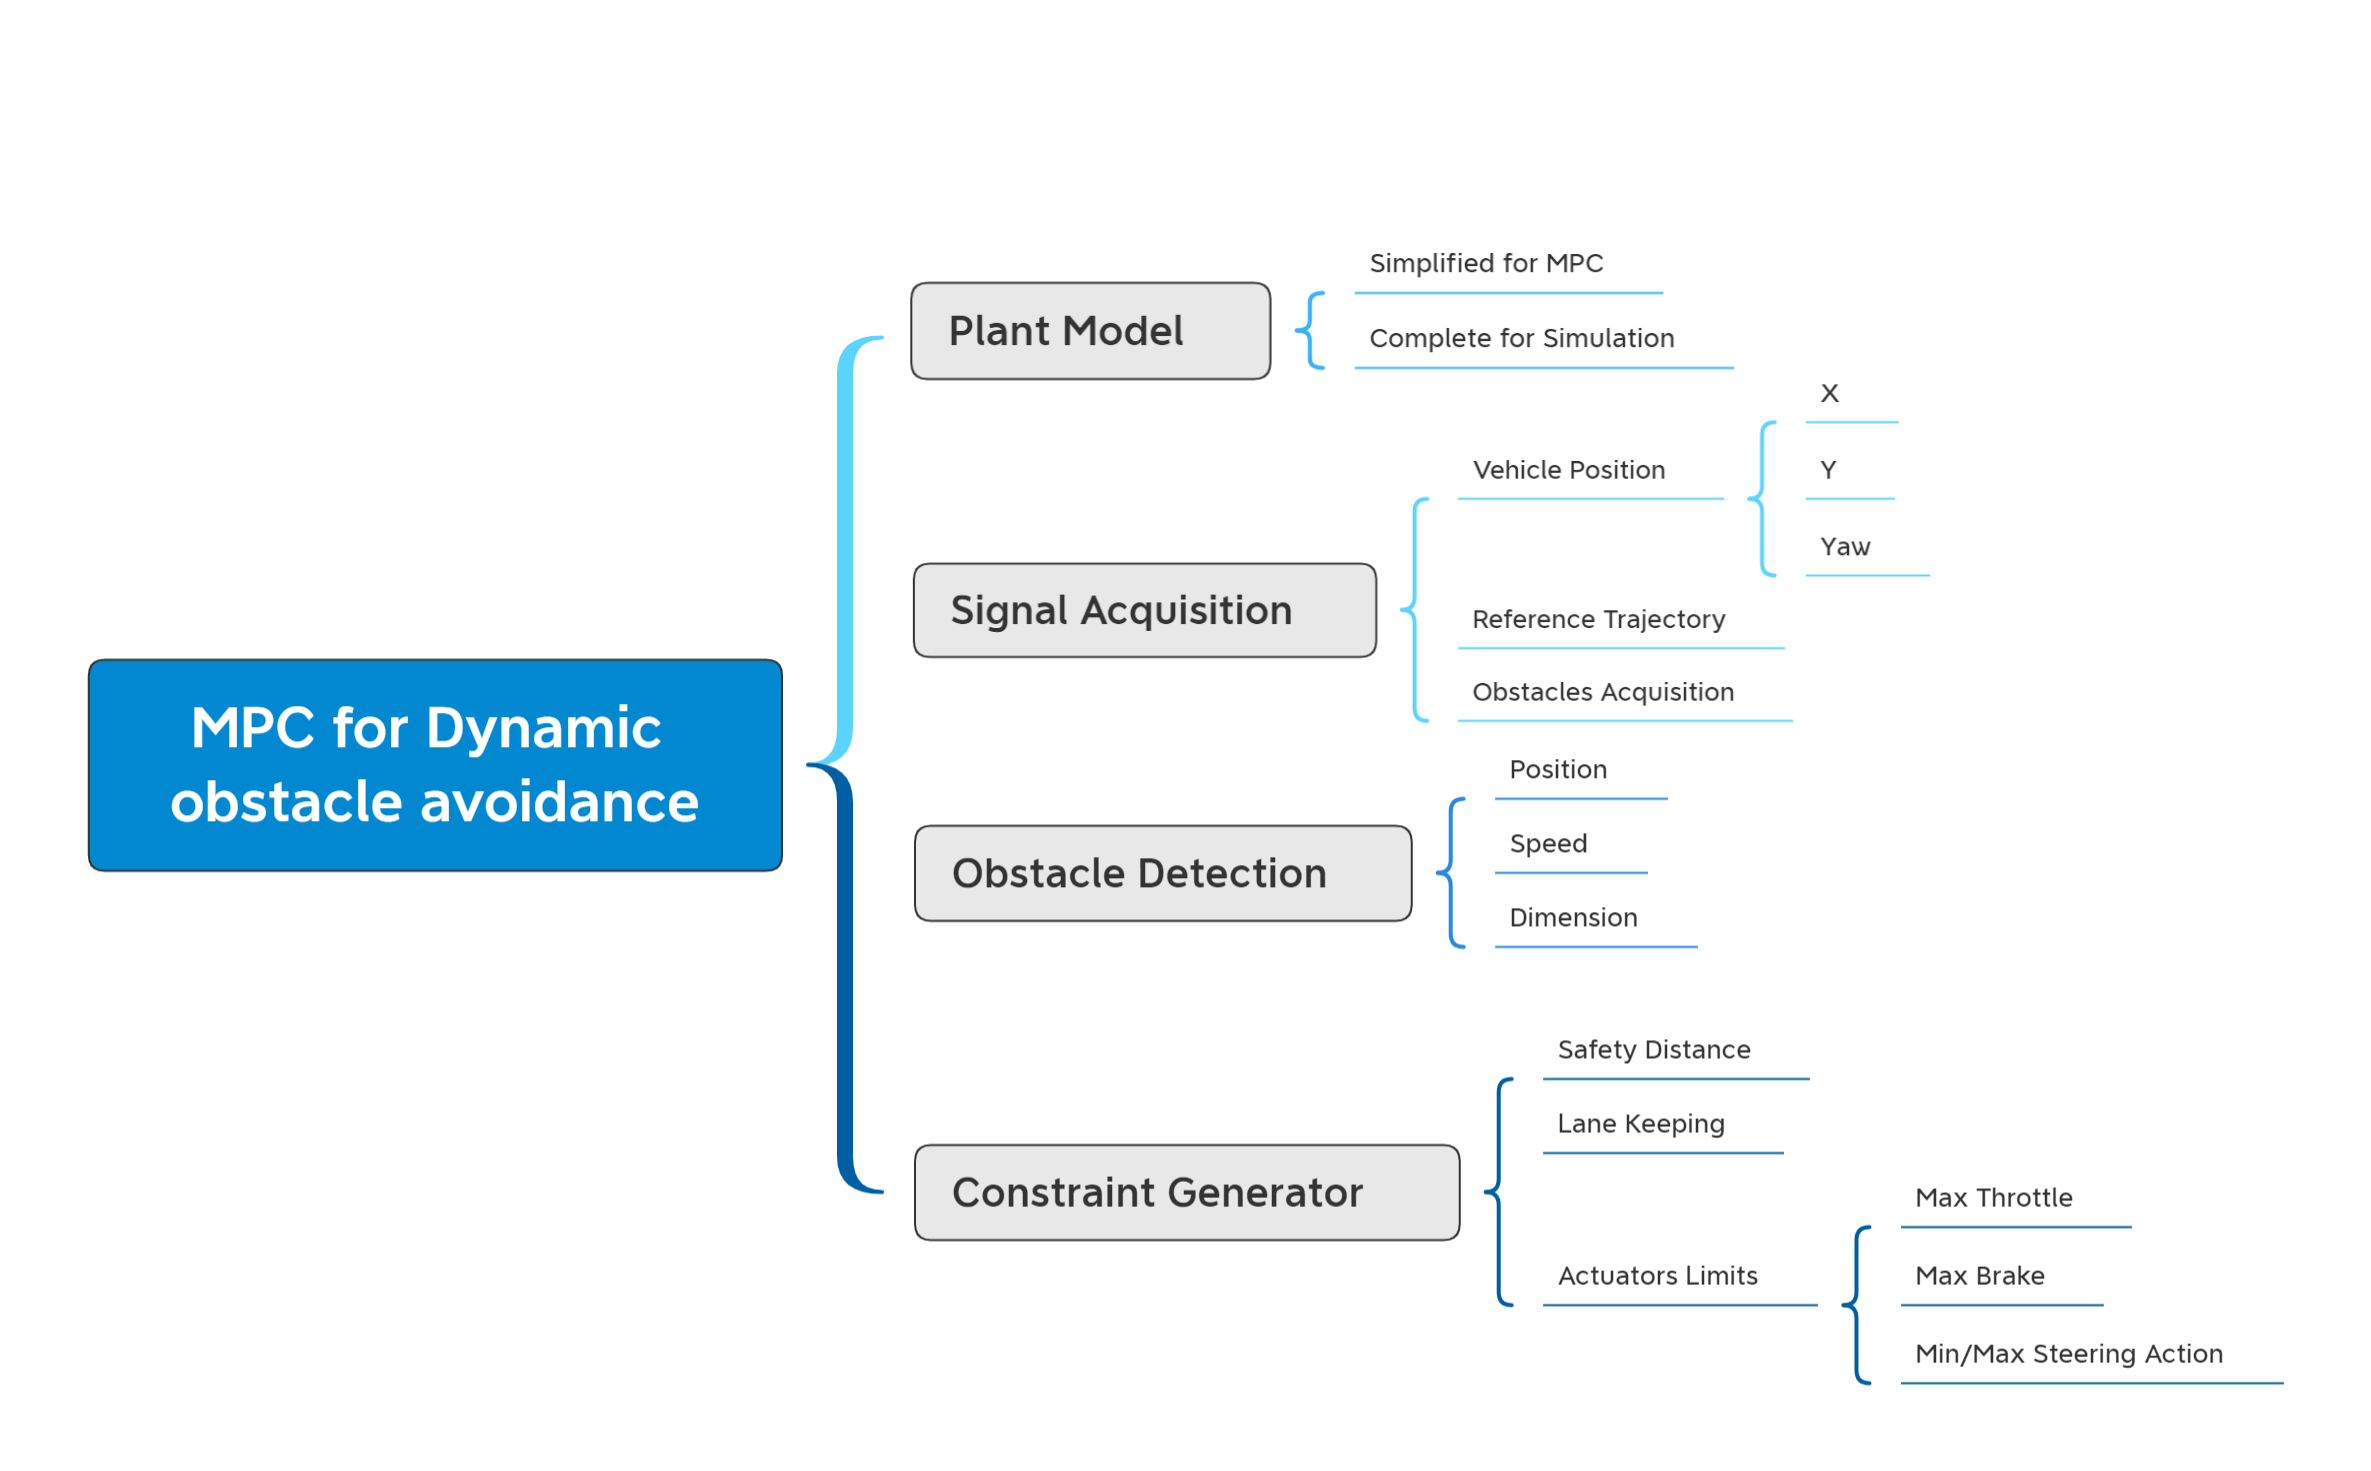
\includegraphics[width=1.25\textwidth,keepaspectratio]{Figures/partitioning.png}}
    \caption{System Partitioning}
    \label{fig:partitioning}
\end{figure}

As shown in the figure above, our project can be divided into four macro-areas:
\begin{itemize}
    \item Plant Model: is the mathematical model of the vehicle which represent the development environment of our project. We have decided to adopt two models, a simplified one to be used in the MPC and a more accurate one to be used in the simulation; 
    \item Signal Acquisition: refers to the gathering of data related to the vehicle position, trajectory, and obstacle acquisition, all coming from the sensors mounted on our vehicle;
    \item Obstacle Detection: here the properties of the obstacle such as position, speed, and dimension  are evaluated;
    \item Constraint Generator: in this phase we set the constraints which the MPC needs to comply with. These constraints are necessary in order to make our model as realistic and safe as possible.
\end{itemize}

These sections will be described in depth in the following chapters.





\section{Plant Model}
\label{chap:Vehicle_model}
The starting point for Model Based design is to develop and implement a plant model, so a model representing the Physics of the system considered.\\
Different models are available in literature to model a vehicle. Since the target of the project is to develop a lateral controller, one of the most suitable model is the so called \textit{Bicycle Model}.\\
The kinematic bicycle model is described by the following non linear system:
\begin{align}
    \dot{X} = Vcos(\psi + \beta)\\
    \dot{Y} = Vsin(\psi + \beta)\\
    \dot{\psi} = \frac{Vcos(\beta)}{l_f + l_r}\left(tan(\delta_f) - tan(\delta_r)\right)\\
    \beta = tan^{-1}\left(\frac{l_ftan(\delta_r) + l_rtan(\delta_f)}{l_f + l_r}\right)
\end{align}
Where:
\begin{itemize}
    \item X and Y are the coordinates of the body of the vehicle in the global reference frame,
    \item $\psi$ is the yaw (orientation angle),
    \item $\beta$ is the slip angle of the body,
    \item $\beta + \psi$ is the body speed direction known as \textit{Course Angle},
    \item $\delta_f$ is the front steering angle,
    \item $\delta_r$ is the rear steering angle,
    \item V is the magnitude of the body speed,
    \item $l_f$ is a geometric parameter which indicates the distance of the CoG from the front wheel,
    \item $l_r$ is a geometric parameter which indicates the distance of the CoG from the rear wheel.
\end{itemize}
\begin{figure}[H]
    \centering
    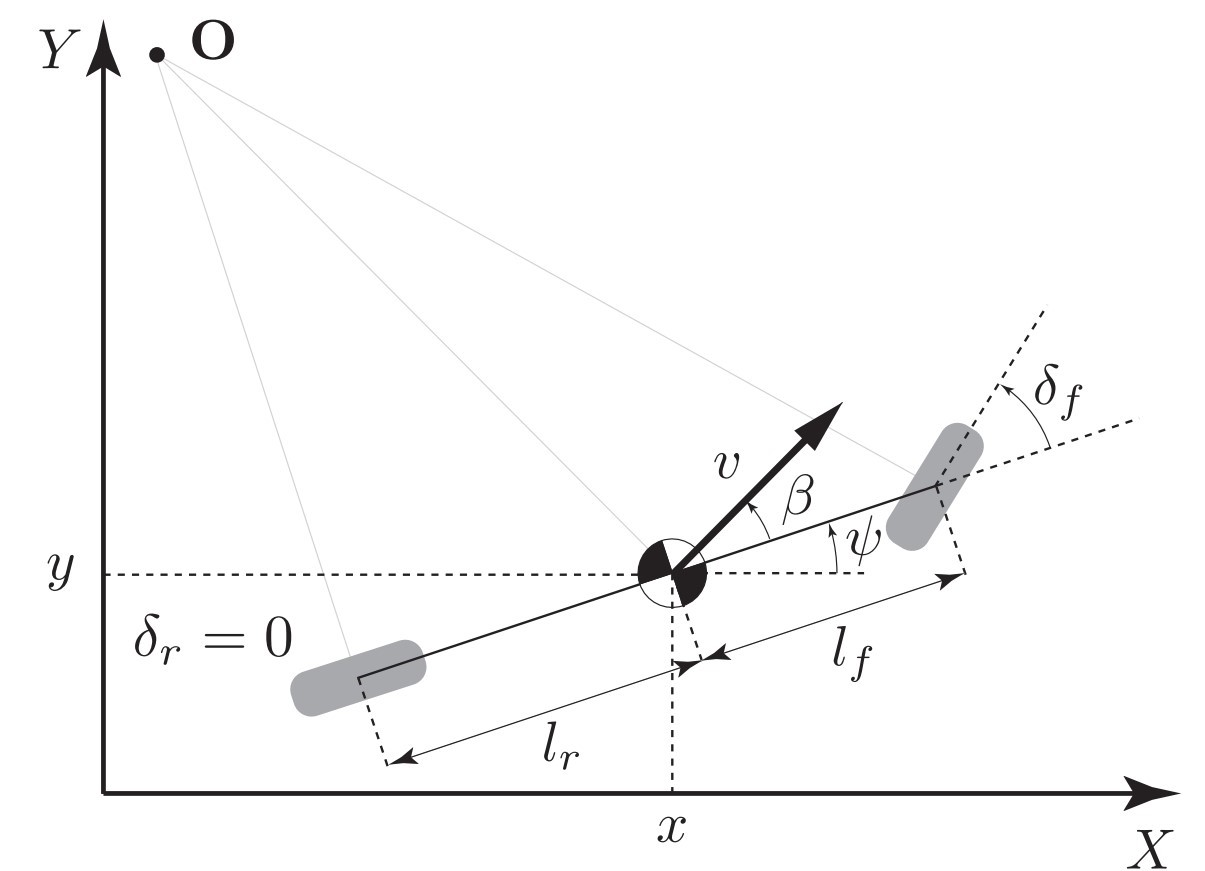
\includegraphics[width=0.5\textwidth]{Figures/Bicycle_model.jpg}
    \caption{Bicycle kinematic vehicle model}
    \label{fig:Bicycle_kin}
\end{figure}
This model can be further simplified assuming that, as in the most of commercial vehicles, only the front wheels are able to steer, so the rear steering angle $\delta_r$ is constant and equal to 0.\\
Standard MPC controller works on linear systems, so we decided to implement a linearized version of the Bicycle Model to feed the controller. This linearized model is described by the following State Space equations:
\begin{equation}
    \label{equation:dynamic1}
    \Dot{x} = Ax + Bu 
\end{equation}
\begin{equation}
    \label{equation:dynamic2}
    y = Cx + Du 
\end{equation}
with:

\begin{equation}
\label{equation:sys_bicycle_kin}
   \begin{aligned}
    x = 
        \begin{bmatrix} % STATES
        X \\ 
        Y \\
        \psi \\
        v \\
        \end{bmatrix}\quad
    A =
        \begin{bmatrix} % MATRIX A
       0 & 0 & -Vsin(\psi) & cos(\psi)\\ 
       0 & 0 & Vcos(\psi) & sin(\psi) \\
       0 & 0 & 0 & \frac{tan(\delta)}{l_r + l_f}\\
       0 & 0 & 0 & 0 \\
        \end{bmatrix}\quad
    B = 
        \begin{bmatrix} % MATRIX B
        0 & 0\\ 
        0 & 0 \\
        0 & \frac{Vtan(\delta)^2 + 1}{l_r + l_f}\\
        1 & 0 \\
        \end{bmatrix}\\[10pt]
    u =
        \begin{bmatrix} % INPUTS
        Throttle \\
        \delta \\
        \end{bmatrix}\quad\quad\quad
    C = I^{4\times 4}\quad\quad\quad\quad\quad
    D =
        \begin{bmatrix} % MATRIX A
      0 & 0 & 0 & 0\\
      0 & 0 & 0 & 0\\
        \end{bmatrix}
    \end{aligned}
\end{equation} 

These matrices are obtained evaluating the Taylor expansion of the non linear bicycle model, as explained in the MathWorks example \cite{StaticObs}.\\
A more complex vehicle model can be useful to test the performance of the controller to be developed. The \textit{Dynamic Bicycle Model} \cite{7225830} can be built starting from the previous non linear model, adding the following equations:
\begin{align}
    \ddot{x} = \dot{\psi}\dot{y} + Throttle\times cos{\psi}\\
    \ddot{y} = -\dot{\psi}\dot{x} + \frac{2}{m}\left(F_fcos(\delta) + F_r\right)\\
    \ddot{\psi} = \frac{2}{I_z}\left(l_fF_f - l_rF_r\right)\\
    \dot{X} = \dot{x}cos(\psi) - \dot{y}sin(\psi)\\
    \dot{Y} = \dot{x}sin(\psi) + \dot{y}cos(\psi)\\
\end{align}
where $m$ is the mass of the vehicle, $I_z$ is the inertia of the vehicle with respect to the vertical axle passing for the CoG of it, while $F_f$ and $F_r$ are respectively the side slip forces acting on the front and rear wheels, and they can be evaluated as:
\begin{align}
    F_f = 2C_f\left(\delta - \theta_f\right)\\
    F_r = 2C_r\left(-\theta_r\right)
\end{align}
with $C_i$ side slip friction coefficient of the i-th wheel couple and $\theta_i$ side slip angle of the wheels.\\
Tyre side slip angles can be approximated by the following equations:
\begin{equation}
    \theta_f=tan^{-1}\left(\frac{\dot{y} + l_f\dot{\psi}}{\dot{x}}\right)
\end{equation}
\begin{equation}
    \theta_r=tan^{-1}\left(\frac{\dot{y} - l_r\dot{\psi}}{\dot{x}}\right)
\end{equation}
The models introduced are, more or less, independent on the longitudinal dynamics of the vehicle, since they link this dynamic with a simple coefficient, that is the $Throttle$. In our model, this coefficient should be considered as an acceleration of the vehicle, and it can be both positive (driving) or negative (braking). Range of values for this parameter is dependent on lots of variables, of course, such as the engine power, the vehicle mass and inertia, the ground type, the rubber of the wheels and so on. Our assumption is to give a fixed interval for this parameter, to simulate a small commercial vehicle on dry asphalt, which can have a maximum acceleration of $4 m/s^2$ and a maximum braking deceleration of $-0.8g$. To summarize:
\begin{itemize}
    \item $Throttle \in [-7.85, 4.00]m/s^2$
    \label{item:Throttle}
\end{itemize}
Parameters considered for the bicycle model are taken from real vehicle data \cite{10.2307/44733900} and are reported in the following table:

\begin{table}[H]
\resizebox{\textwidth}{!}{%
\begin{tabular}{|l|l|r|r|r|r|r|}
\hline
\textbf{ID} &
  \textbf{Vehicle name} &
  \multicolumn{1}{l|}{\textbf{Wheel base {[}$m${]}}} &
  \multicolumn{1}{l|}{\textbf{l\_r {[}$m${]}}} &
  \multicolumn{1}{l|}{\textbf{l\_f {[}$m${]}}} &
  \multicolumn{1}{l|}{\textbf{Mass {[}$kg${]}}} &
  \multicolumn{1}{l|}{\textbf{Inertia {[}$kg \cdot m^2${]}}} \\ \hline
1 & \textit{Hyundai Azera }    & 2.843 & 1.738 & 1.105 & 1200 & 1000 \\ \hline
2 & \textit{BMW 325i}          & 2.570 & 1.369 & 1.201 & 1251 & 2027 \\ \hline
3 & \textit{Ford E150 }        & 3.505 & 1.634 & 1.871 & 2995 & 6536 \\ \hline
4 & \textit{Suzuki Samurai}    & 2.032 & 0.870 & 1.162 & 1229 & 1341 \\ \hline
5 & \textit{Volkswagen Beetle} & 2.408 & 0.996 & 1.412 & 857  & 1289 \\ \hline
\end{tabular}%
}
\caption{Vehicle data considered for development and validation}
\label{tab:vehicle_data}
\end{table}
Values reported in the table \ref{tab:vehicle_data} are stored in a MATLAB file and can be accessed through the \textit{loadParameters} function, which take as input the vehicle ID and returns the parameters associated with that vehicle. To avoid to call improperly this function, a default parameters set as been provided with the following values:
\begin{table}[H]
\resizebox{\textwidth}{!}{
\begin{tabular}{|l|r|r|r|r|r|}
\hline
\textbf{Vehicle name} &
  \multicolumn{1}{l|}{\textbf{Wheel base {[}$m${]}}} &
  \multicolumn{1}{l|}{\textbf{l\_r {[}$m${]}}} &
  \multicolumn{1}{l|}{\textbf{l\_f {[}$m${]}}} &
  \multicolumn{1}{l|}{\textbf{Mass {[}$kg${]}}} &
  \multicolumn{1}{l|}{\textbf{Inertia {[}$kg \cdot m^2${]}}} \\ \hline
\textit{Default}    & 2 & 1 & 1 & 1000 & 1000 \\ \hline
\end{tabular}
}
\end{table}
We used data of vehicle 1, \textit{Hyundai Azera}, for the development phase, where mass and inertia are not the real ones of the vehicle, but are given with realistic values, while other data of the previous table \ref{tab:vehicle_data} are meant to be used in the validation phase, to test the controller with different vehicles.
For what concern the side slip friction values, we considered two fixed values for all the vehicles that are:
\begin{itemize}
    \item $C_f$ $=$ $1.0745\times10^5$ N/rad
    \item $C_r$ $=$ $1.9032\times10^5$ N/rad
\end{itemize}
while in the \textit{"default"} condition they are both $10^5$ N/rad.

\subsection{Model comparison}
As specified in the subsection \ref{partitioning_subsection} we have decided to use two models, a simplified and linearized model for the MPC and a more complex one for the simulation of the model. The former is defined as \textit{Kinematic Bicycle Model} and the latter as \textit{Dynamic Bicycle Model}.
Hence we have decided to test both of these systems to show how they behave with different throttle and steering inputs using the \textit{Simulink Test} tool. Thus, the tests performed are:
\begin{itemize}
    \item \textbf{Free evolution test}: this test has been performed considering a constant steering of $0^{\circ}$ and a constant throttle of 0 $m/s^2$;
    \item \textbf{Only throttle test}: this test has been performed keeping the steering angle constant and equal to $0^{\circ}$ and varying the throttle as shown in Figure \ref{fig:InputThrottle};
    \item \textbf{Constant steering test}: this test has been performed keeping the throttle constant and equal to 0 $m/s^2$ and the steering angle constant and equal to $2^{\circ}$;
    \item \textbf{Ramp steering test}: this test has been performed keeping the throttle equal to 0 $m/s^2$ and giving a ramp steering angle signal (varying linearly from $0^{\circ}$ to $36^{\circ}$);
    \item \textbf{Small sinusoidal steering test}: this test has been performed keeping the throttle constant and equal to 0 $m/s^2$ and giving a sinusoidal steering angle signal with frequency 0.2 $Hz$ and amplitude $5^{\circ}$;
    \item \textbf{Big sinusoidal steering test}: here we have performed the same test as before (sinusoidal steering input) but with a larger amplitude of the sine wave ($15^{\circ}$);
    \item \textbf{Combined test 1}: this test has been performed keeping the steering angle constant and equal $2^{\circ}$ and varying the throttle as shown in Figure \ref{fig:InputThrottle};
    \item \textbf{Combined test 2}: this test has been performed keeping the throttle equal to 0.2 $m/s^2$ and giving a ramp steering angle signal (varying linearly from $0^{\circ}$ to $36^{\circ}$).
\end{itemize}

\begin{figure}[H]
    \centering
    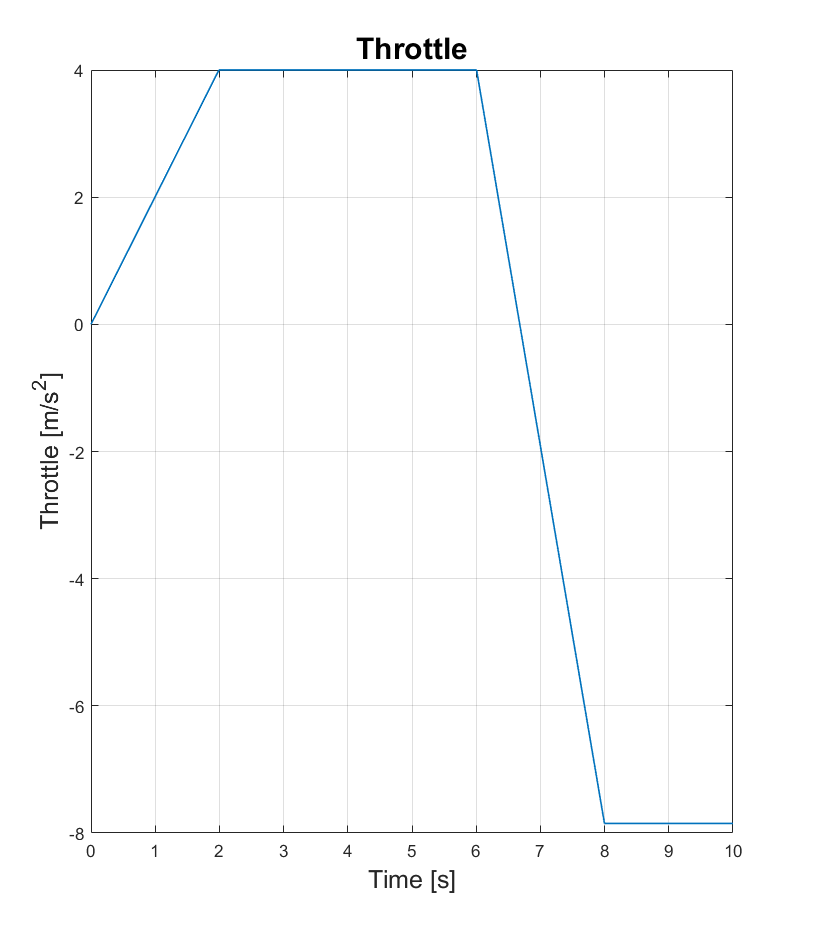
\includegraphics[width=0.65\textwidth]{Figures/InputThrottle.png}
    \caption{Throttle Input used in \textit{Only throttle test} and \textit{Combined test 1}. Maximum and minimum values are coherent with the range described in Section \ref{item:Throttle} in order to explore the whole set of throttle values.}
      \label{fig:InputThrottle}
\end{figure}






\subsubsection{Simulink Test}
The above-mentioned tests have been performed using the \textit{Simulink Test} tool implemented by MathWorks. Simulink Test provides tools for authoring, managing, and executing systematic, simulation-based tests of models, generated code, and simulated or physical hardware. It includes simulation, baseline, and equivalence test templates that let you perform functional, unit, regression, and back-to-back testing using software-in-the-loop (SIL), processor-in-the-loop (PIL), and real-time hardware-in-the-loop (HIL) modes. With Simulink Test you can create non-intrusive test harnesses to isolate the component under test. You can define requirements-based assessments using a text-based language, and specify test input, expected outputs, and tolerances in a variety of formats. \cite{SimulinkTest}

\subsubsection{Results analysis}

Exploiting Simulink Test, we have created two test harnesses : \textit{Dynamic} and \textit{Kinematic}. Those are referred to the models described at the beginning of this section. Then, we have executed an Equivalence Test which allowed us to make a comparison between two simulations. In particular, the Dynamic Model has been considered as the \textit{baseline} which our Kinematic Model has been compared to in the test. The baseline represents the expected output being more accurate than the Kinematic model, which in turn is called \textit{Compare to} model inside the Simulink Test automatic report generator\footnote{The ``Model Comparison - Test Report" file generated by Simulink Test is included in the /Documentation/Test Reports/ file path}. 
Since these tests aim to give a qualitative analysis of the two models and compare them, we have not included equivalence criteria.
The only parameter we have set up is the relative tolerance assigning to it a value of 1\% in order to ignore the negligible offsets between the dynamic model and the kinematic model.\\
Figure \ref{fig:trajectories} shows the results of the simulations we have carried out. 
As shown in Figures \ref{subfig:free_evo} and \ref{subfig:only_throttle} respectively, as expected the two models behave in the same way when no inputs are present or when only the longitudinal input (throttle) is changed. \\ Another relevant result is shown in Figures \ref{subfig:small_sinusoidal} and \ref{subfig:big_sinusoidal}: as long as the amplitude of the sinusoidal input is fairly small, the two models behave in a similar fashion but the greater the amplitude of the sinusoidal input, the greater the deviation of the kinematic model from the dynamic one.\\
The other images shown below, underline as well the offset between the two vehicle models, which is due to the fact that when using the dynamic model we take into account lateral slips which are not considered in the kinematic model.


\begin{figure}[H]
\centering

    \begin{subfigure}{.5\textwidth}
    \centering
   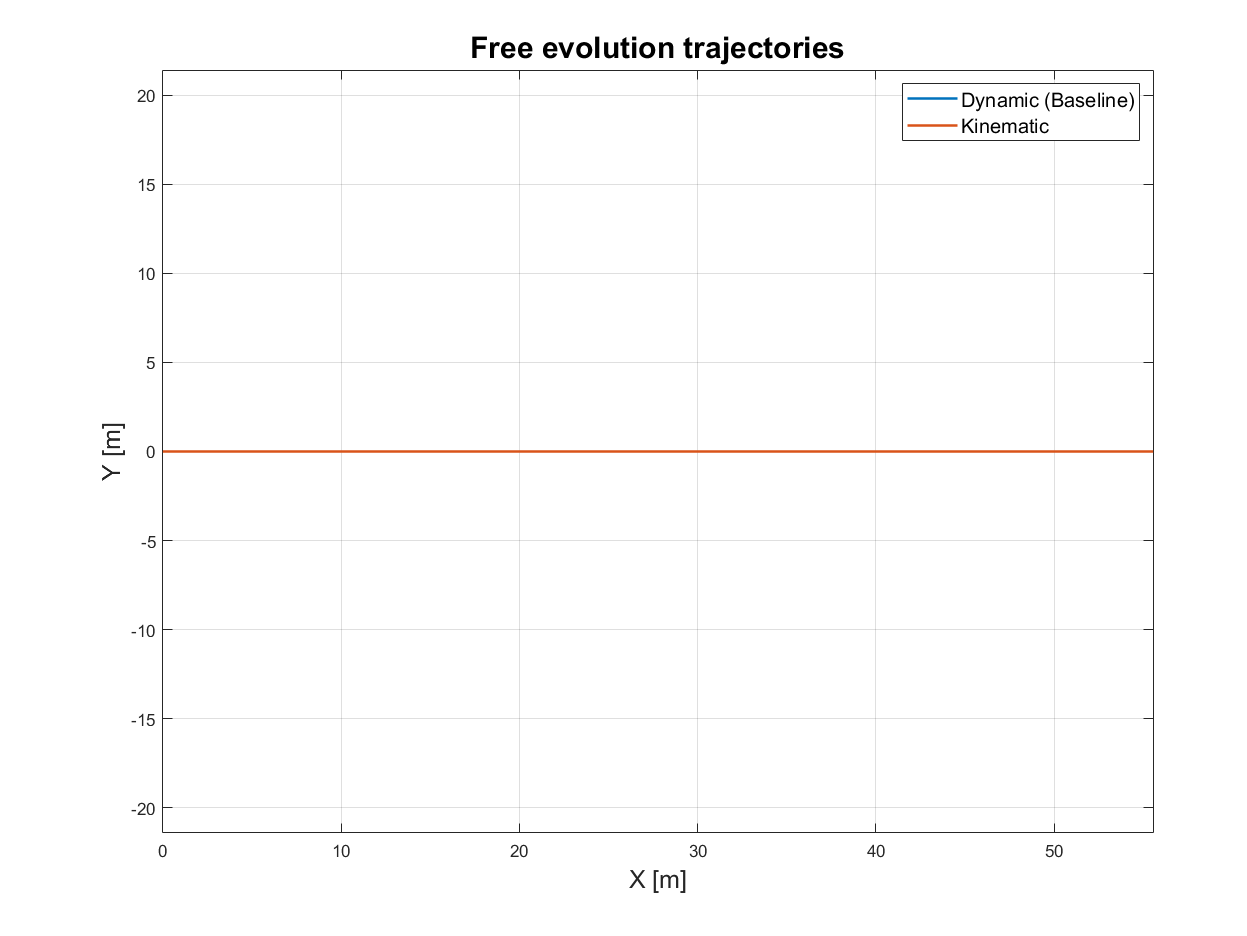
\includegraphics[width=1.1\textwidth,keepaspectratio]{Figures/Free_evo_traj.png}
    \caption{Free evolution test - trajectories}
    \label{subfig:free_evo}
    \end{subfigure}%
    \begin{subfigure}{.5\textwidth}
    \centering
    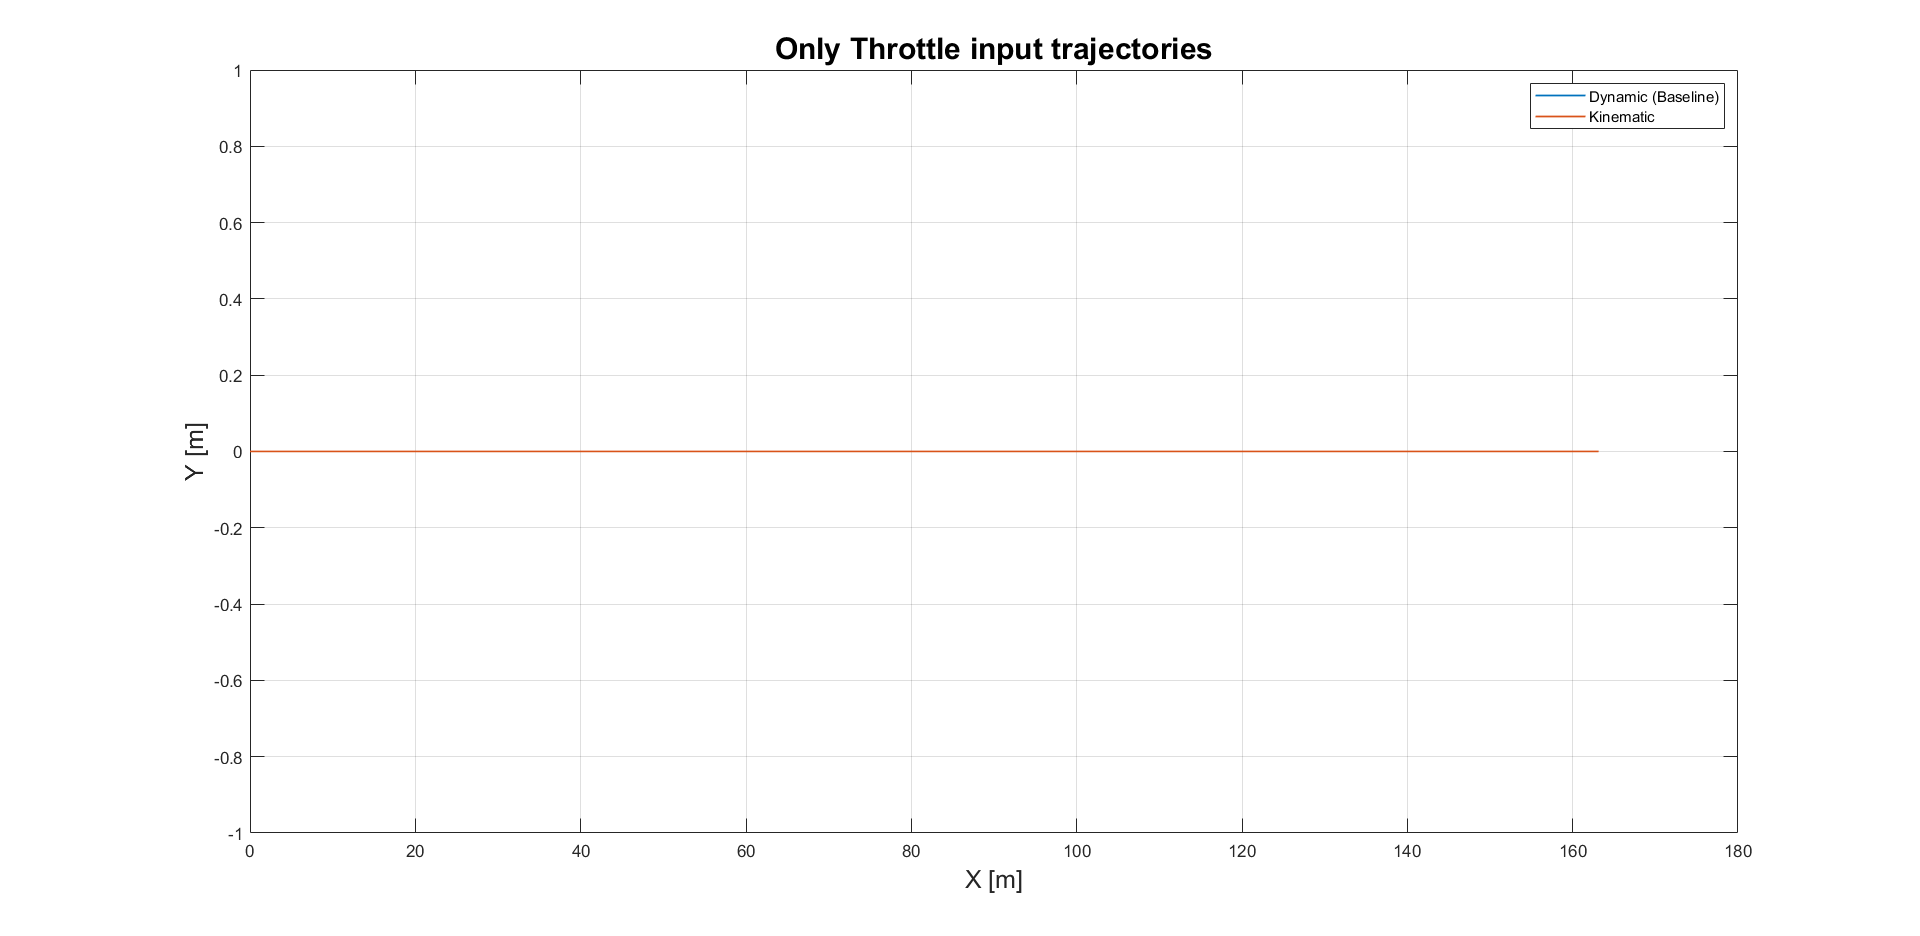
\includegraphics[width=1.1\textwidth,keepaspectratio]{Figures/Throttle_traj.png}
    \caption{Only throttle test - trajectories}
    \label{subfig:only_throttle}
    \end{subfigure}
    
    \vspace{10mm}
    
    \begin{subfigure}{.5\textwidth}
    \centering
   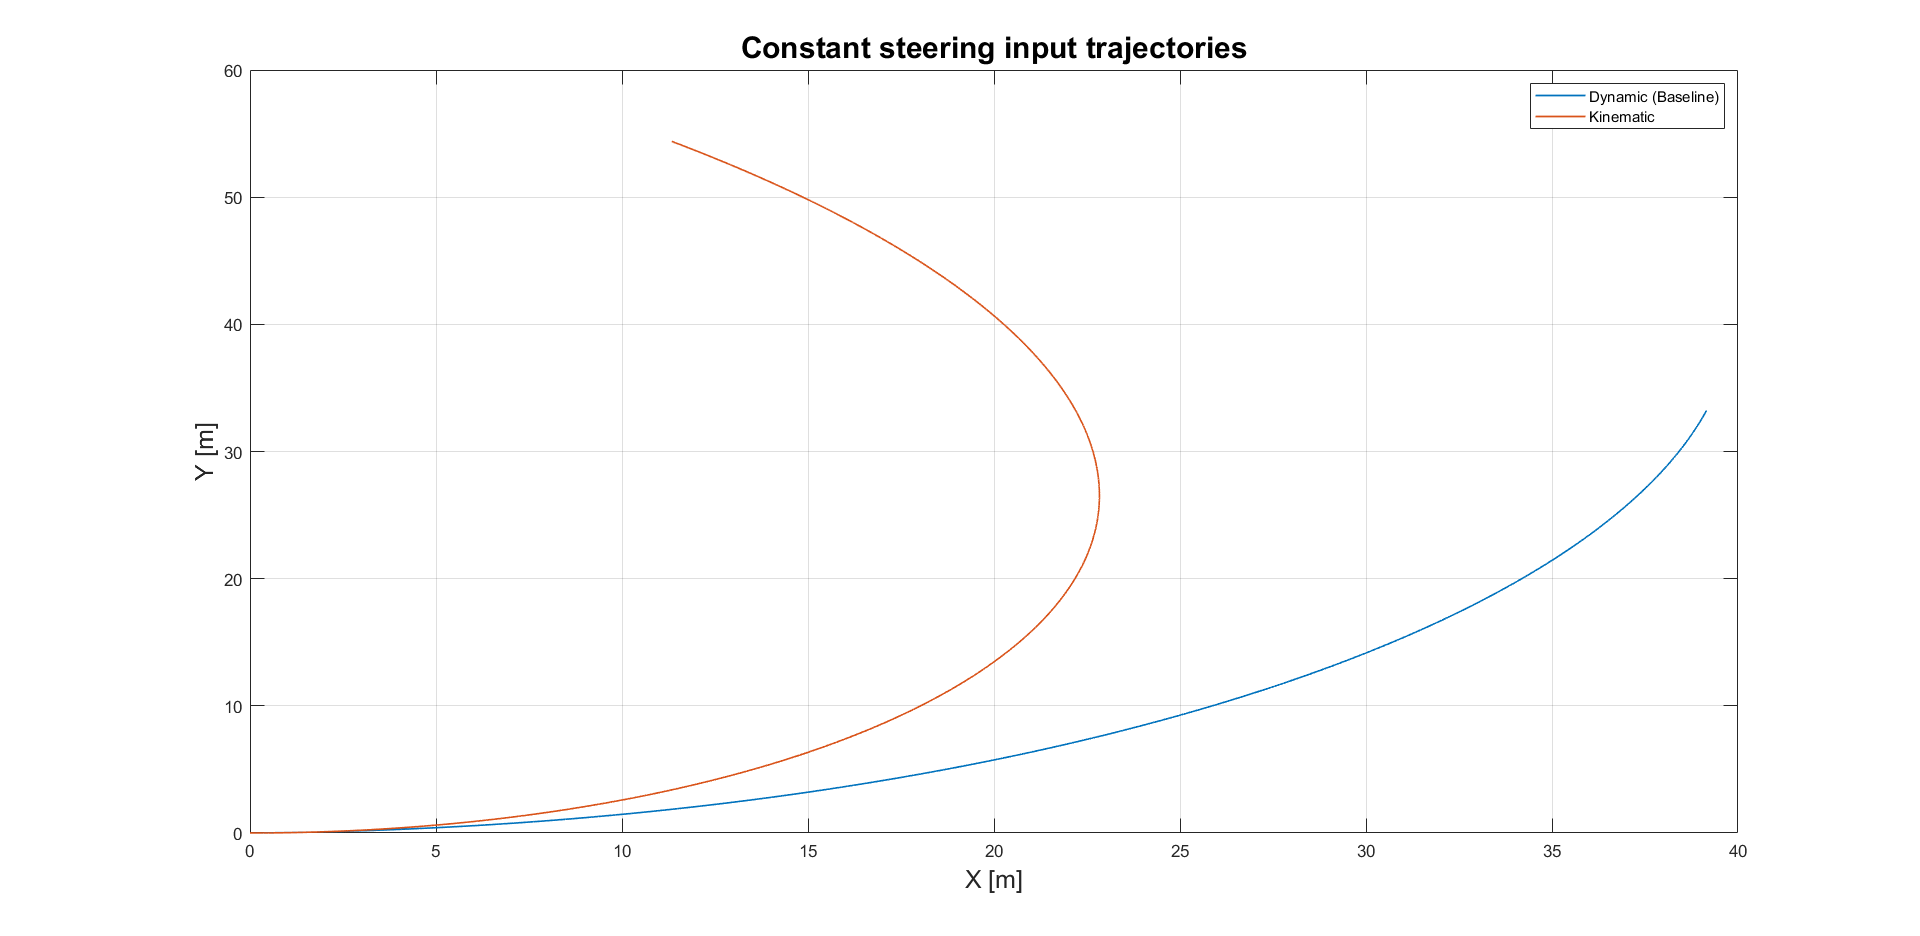
\includegraphics[width=1.1\textwidth,keepaspectratio]{Figures/Const_steer_traj.png}
   \caption{Constant steering test - trajectories}
   \label{subfig:const_steer}
    \end{subfigure}%
    \begin{subfigure}{.5\textwidth}
    \centering
    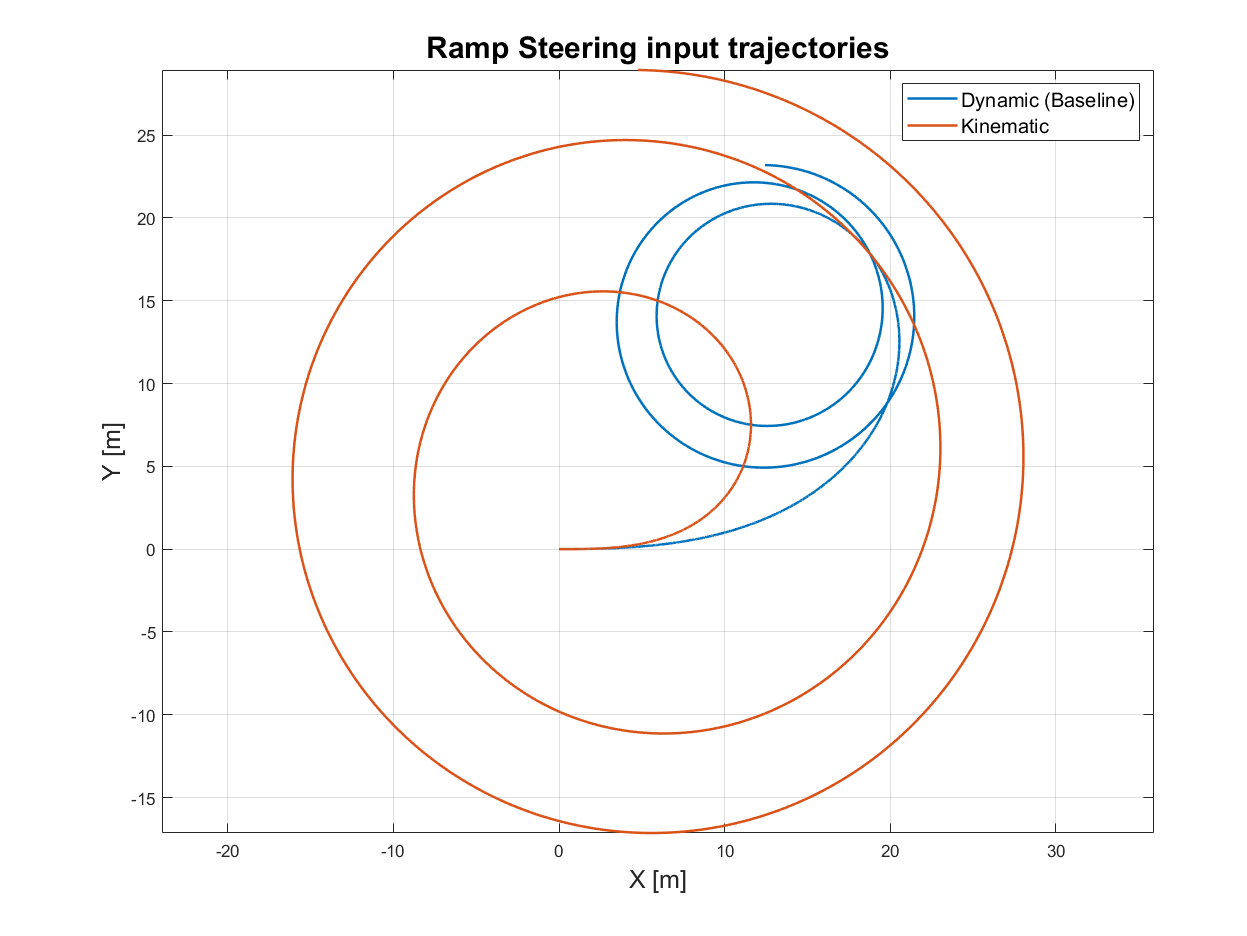
\includegraphics[width=1.1\textwidth,keepaspectratio]{Figures/Ramp_traj.png}
    \caption{Ramp steering test - trajectories}
    \label{subfig:ramp_steer}
    \end{subfigure}
    
     \vspace{10mm}
     
    \begin{subfigure}{.5\textwidth}
    \centering
   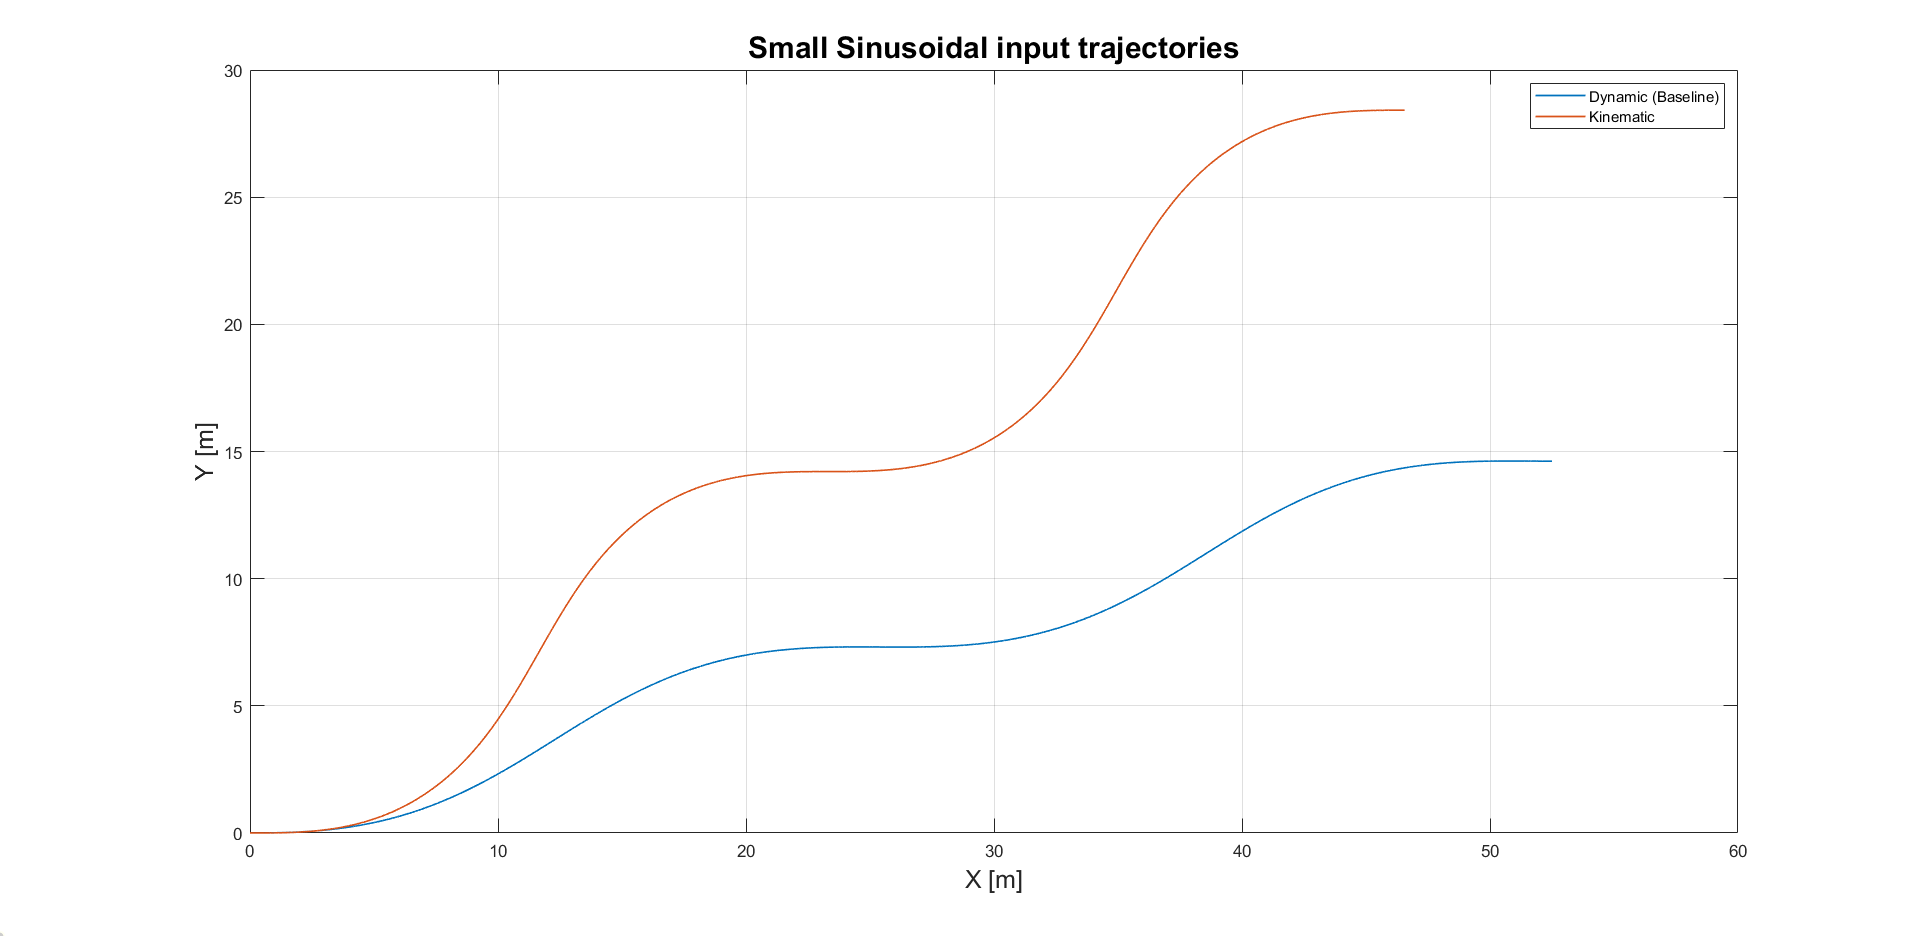
\includegraphics[width=1.1\textwidth,keepaspectratio]{Figures/Small_sin_traj.png}
   \caption{Small sinusoidal test - trajectories}
   \label{subfig:small_sinusoidal}
    \end{subfigure}%
    \begin{subfigure}{.5\textwidth}
    \centering
    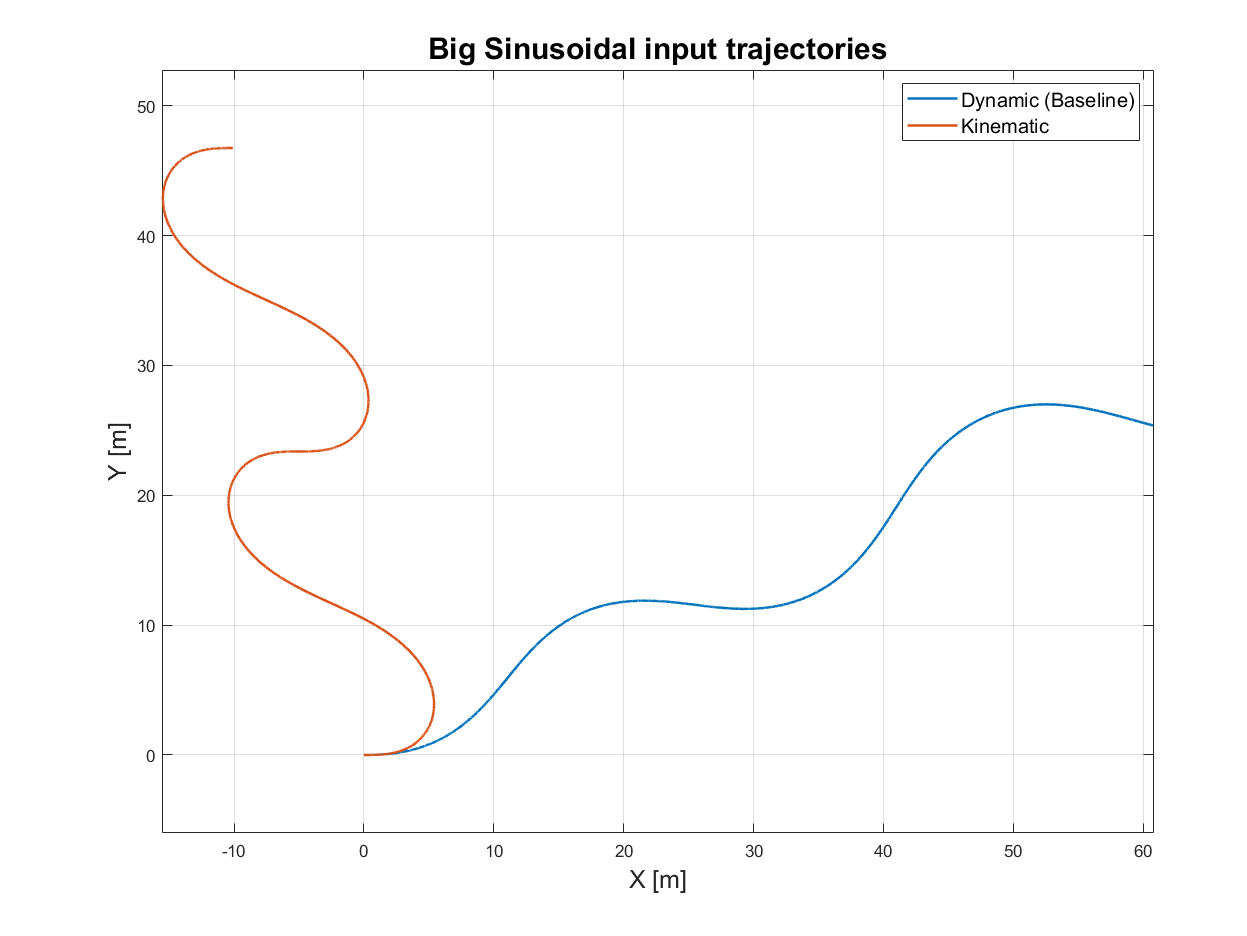
\includegraphics[width=1.1\textwidth,keepaspectratio]{Figures/Big_sin_traj.png}
    \caption{Big sinusoidal test - trajectories}
    \label{subfig:big_sinusoidal}
    \end{subfigure}
    
     \vspace{10mm}
    
    \begin{subfigure}{.5\textwidth}
    \centering
  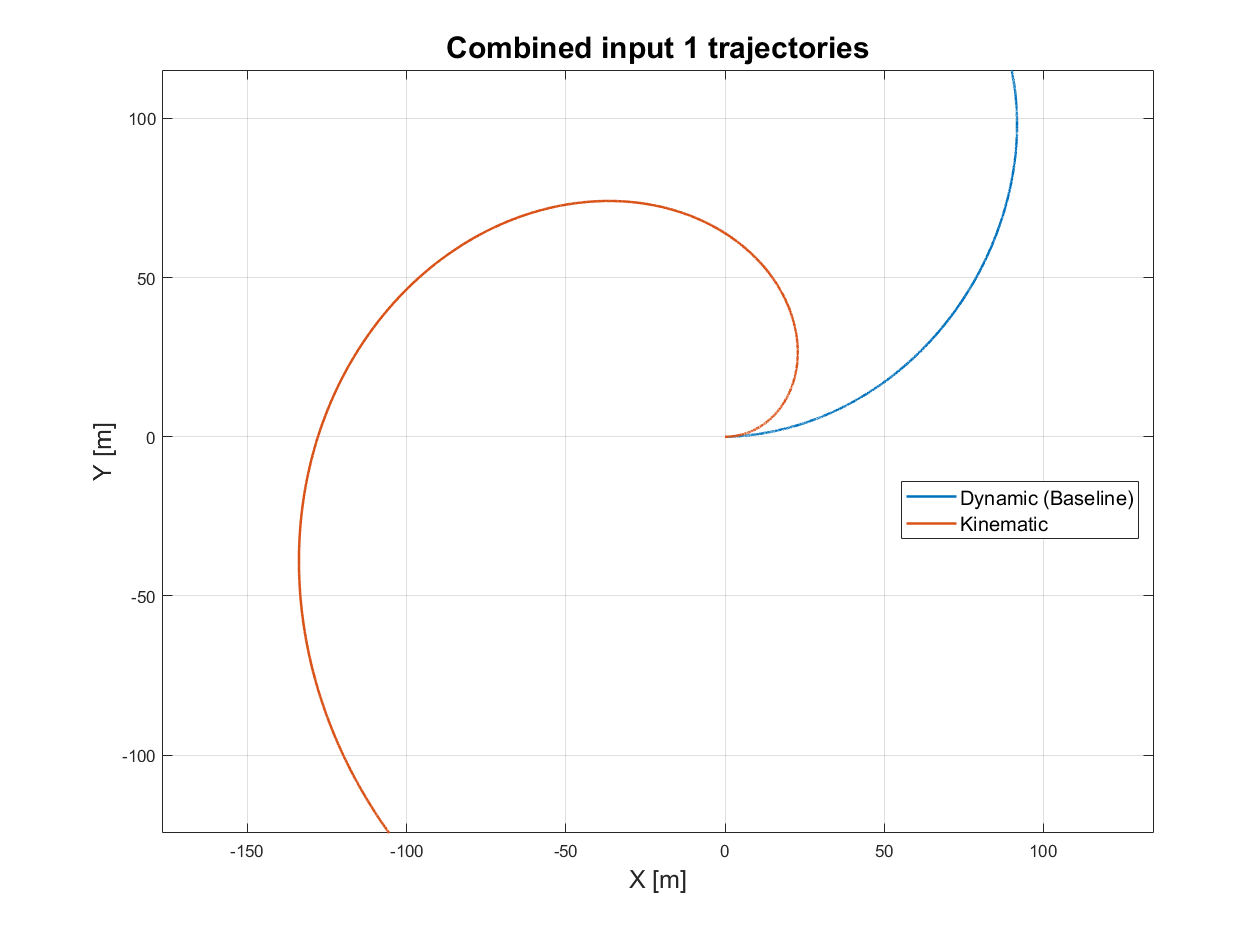
\includegraphics[width=1.1\textwidth,keepaspectratio]{Figures/Comb1_traj.png}
    \caption{Combined 1 test - trajectories}
    \label{subfig:Comb_1}
    \end{subfigure}%
    \begin{subfigure}{.5\textwidth}
    \centering
  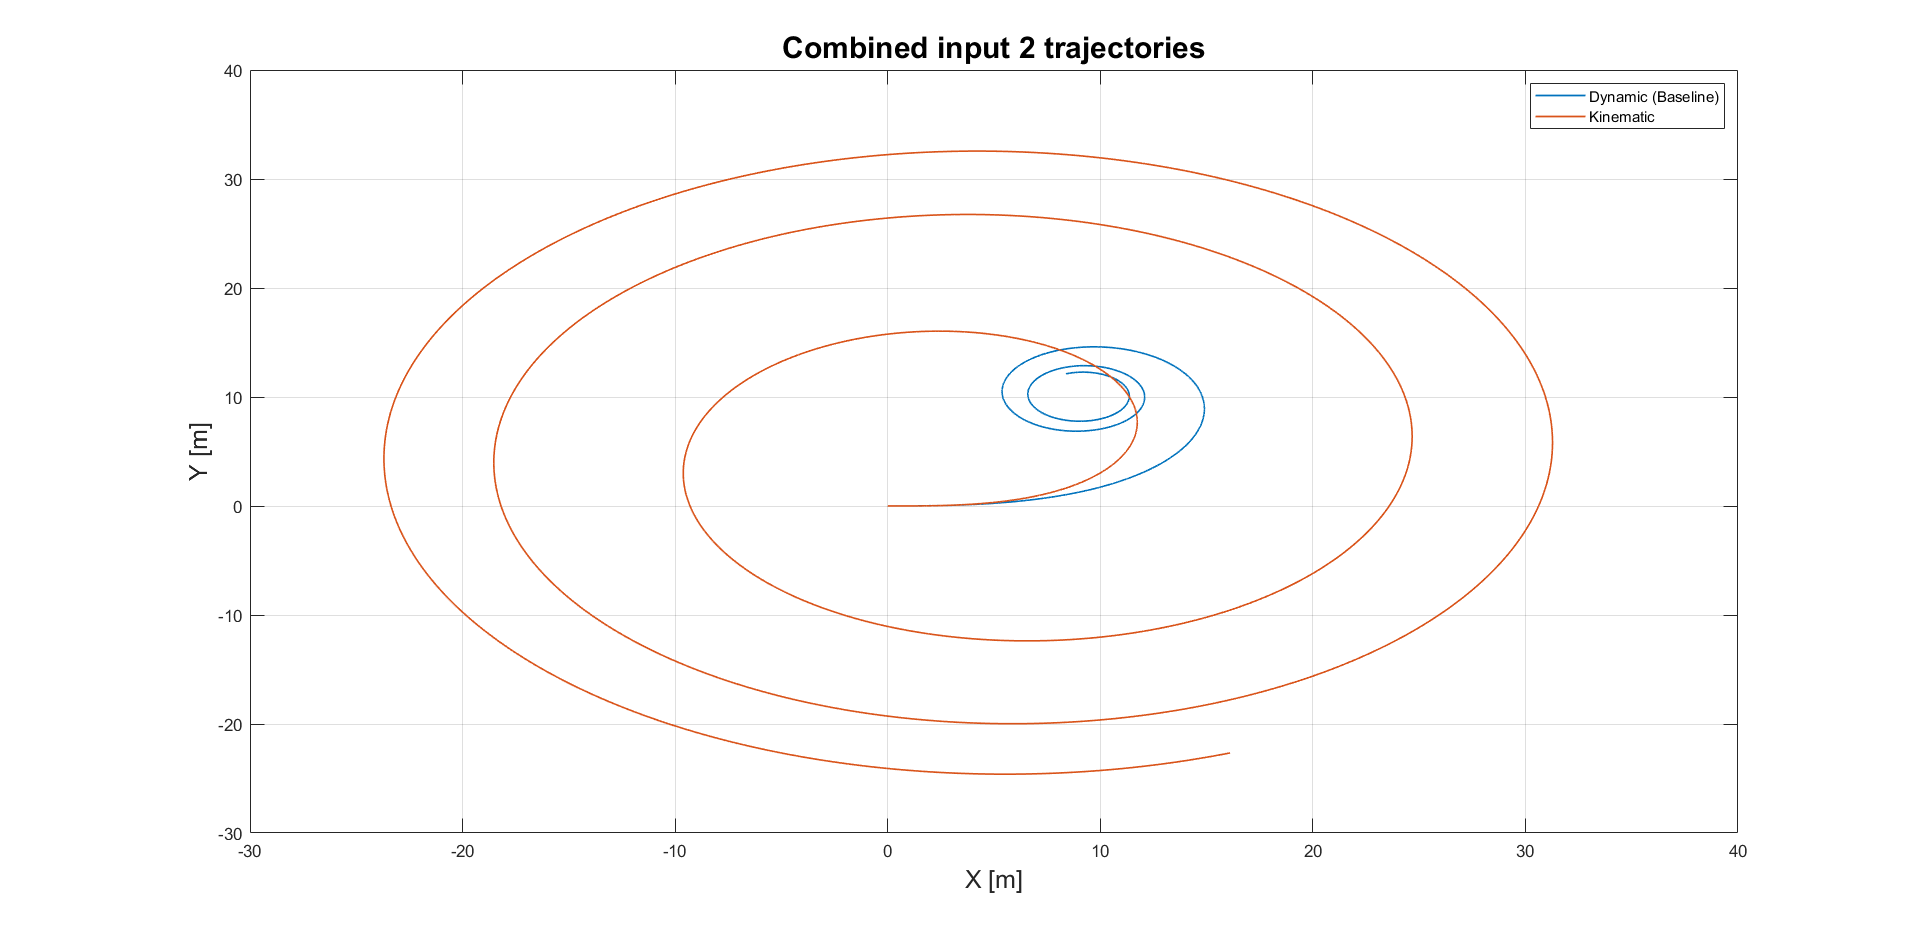
\includegraphics[width=1.1\textwidth,keepaspectratio]{Figures/Comb2_traj.png}
    \caption{Combined 2 test - trajectories}
    \label{subfig:Comb_2}
    \end{subfigure}
    
    \caption{Output trajectories of the test set}
    \label{fig:trajectories}
\end{figure}
\pagebreak


After the analysis of the results, we decided to provide to the MPC the linearized bicycle model for the vehicle plant, because the controller is usually updated with the current state in some fractions of a second, and for this reason the differences between the model and the \textit{``Real World"} system, that in our case is represented by the dynamic model, shouldn't affect too much the behaviour of the controller itself. As a matter of fact, by looking at the images above it is clear that the difference between the two models output is negligible at the first time steps of the simulation.\\
Moreover, as already discussed in this section, the performances of the two models are very similar if compared with small inputs, and this condition is fulfilled if we consider to use our controller in normal driving scenarios, such as, for instance, an highway.\\
Keeping in mind these assumptions, we go on with the project, considering to apply a change in the vehicle model for the MPC if we are not able to achieve good results with this one.
\section{Signal Acquisition} 
\label{chap:SignalAcquisition}
All autonomous vehicles must have a sufficient knowledge of the surrounding environment and obtain accurate location information. For this purpose different sensors need to be adopted on a single vehicle, as a matter of fact different sensor have different limitations which can be overcome through sensor fusion. This approach is able to compensate the limitations of one sensor with the strengths of another.
%%%%%%%%%%%%%%%%%%%%%%%%%%%%%%%%%%%%%%%%%%
\subsection{Sensors used in obstacle avoidance}
When dealing with autonomous driving, three are the core functions of interest: 
\begin{itemize}
    \item perception: visual perception (e.g., camera) and radar perception (e.g., LIDAR);
    \item planning: GPS, Inertial Navigation System (INS), and HD Maps;
    \item control: image identification, deep learning and artificial neural networks.
\end{itemize}

\subsection{Perception: what a self-driving car sees}
The three primary autonomous vehicle sensors for perception are camera, radar and lidar. Working together, they provide the car visuals of its surroundings and help it to detect the speed and distance of nearby objects, as well as their three-dimensional shape. \cite{NVIDIA}

\subsubsection{Camera} 
Cameras are the main type of sensors for creating a visual representation of the surrounding world, as a matter of fact autonomous vehicles rely on cameras placed on every side to stitch together a 360 degrees view of their environment.
Though providing very accurate images up to 80 meters, cameras have limitations:
\begin{itemize}
    \item the distance from target objects needs to be calculated in order to know exactly where they are;
    \item mechanical issues: mounting multiple cameras as well as keeping them clean;
    \item issues related to low visibility conditions (e.g., rain, fog, nighttime);
    \item heavy graphic processing needed.
\end{itemize}

\subsubsection{Radar} \label{radar}
Radars can overcome cameras limitations in low visibility scenarios and improve object detection.
The working principle of radars is based on radio pulses emitted by a source. Once these pulses hit an object they travel back to the sensor providing information about its speed and location. 
The maximum distance range for radar-based sensors is 250 meters for Long-Range Radars, 100 meters for Medium-Range Radars and 30 meters for Short-Range Radar.

\subsubsection{Lidar}
The name LiDAR stands for Light Detection and Ranging and its working principle is analogous to the radar's (Sub-section \ref{radar}) but using a different part of the electro-magnetic spectrum. Radars use radio waves or microwaves while lidars use light near the visible spectrum.
This type of sensors make it possible for an autonomous car to create a 3D point cloud map and they provide shape and depth of the surroundings and its actors.

\subsection{Planning: know where a self-driving car is going}

\textit{``As the core of the planning layer, localization and navigation technologies including GPS, INS, and HD maps aim to assist self-driving cars in planning routes and navigating in real time."} \cite{luo2019localization}

\vspace{2mm}

The above-mentioned technologies which have to be always active, allow the vehicle to go from point A to point B following the optimal route, and must re-compute in real-time the path if the optimal one has any unexpected diversions using a well tuned controller.

\subsubsection{GPS}
GPS stands for Global Positioning System. A GPS receiver is able to compute the current position of the vehicle together with the current time, acquiring and analysing signals received from at least four of the constellation of over 60 low-orbit satellites. 
The accuracy on the position information is 1 meter.

\subsubsection{INS}
INS stands for Inertial Navigation System and allows the accurate sensing of high-precision 3D position, velocity, and attitude information of the car via the inertial measurement unit (IMU).
It can make up for the deficiency of GPS localization, which is not real-time enough.

\subsubsection{HD Maps}
HD Maps are crucial when it comes to Self-Driving Vehicles, these high-definition 3D maps are highly accurate and contain details not normally present on traditional maps. Such maps can be precise at a centimetre level.
HD Maps consist of two map layers: static and dynamic HD Map.
The former is usually collected in advance and contains lane models, road information, and road attributes while the latter, stored on a cloud platform, contains real-time traffic information. Moreover, dynamic HD Maps can be updated in real-time through information collected from vehicles and infrastructures on the cloud.

\subsection{Our Assumptions}

Our model is based on several assumptions regarding data acquisition from the sensors and how these data are translated into useful information. Below the list of assumptions we have made:
\begin{itemize}
    \item we suppose no error in the information collected from the sensors;
    \item our car knows all the information related to the road model, such as lane width and number of lanes by acquiring them from cameras installed on the vehicle and HD Maps;
    \item the vehicle knows its position in the XY reference frame, through the use of GPS and INS;
    \item the route planning done by our controller exploits the latitude and longitude information to plan out a complete route based on the HD Maps, GPS, and INS. Moreover, while driving, the car also compares the HD maps with the perception information from sensors to get changing environment information for dynamically planning routes and making decisions;
    \item we suppose to have both a Long-Range Radar and Lidar mounted on the vehicle, hence to be able to detect obstacles in the range of 200 meters together with their velocities.
\end{itemize}

Though we include all the above information on the MATLAB code, we suppose to collect them using sensors, as previously described.







%%%%%%%%%%%%%%%%%%%%%%%%%%%%%%%%%%%%%%%%%%

\subsection{Reference trajectory}
After implementing the vehicle model and keeping in mind the assumptions made above, we have generated and imposed a reference trajectory to the vehicle in order to have a path to follow during the development and the testing phases.
To do so, we have taken the desired scenario from a real map using the open source website \href{https://www.openstreetmap.org}{\textit{OpenStreetMap}}\cite{OpenStreetMap} (Figure \ref{fig:OpenStreetMap}).
The website allows the user to export any route as a \textit{.osm} file containing the global coordinates of the area together with some useful metadata such as street name, number of lanes, speed limits, etc.

\begin{figure}[H]
    \centering
    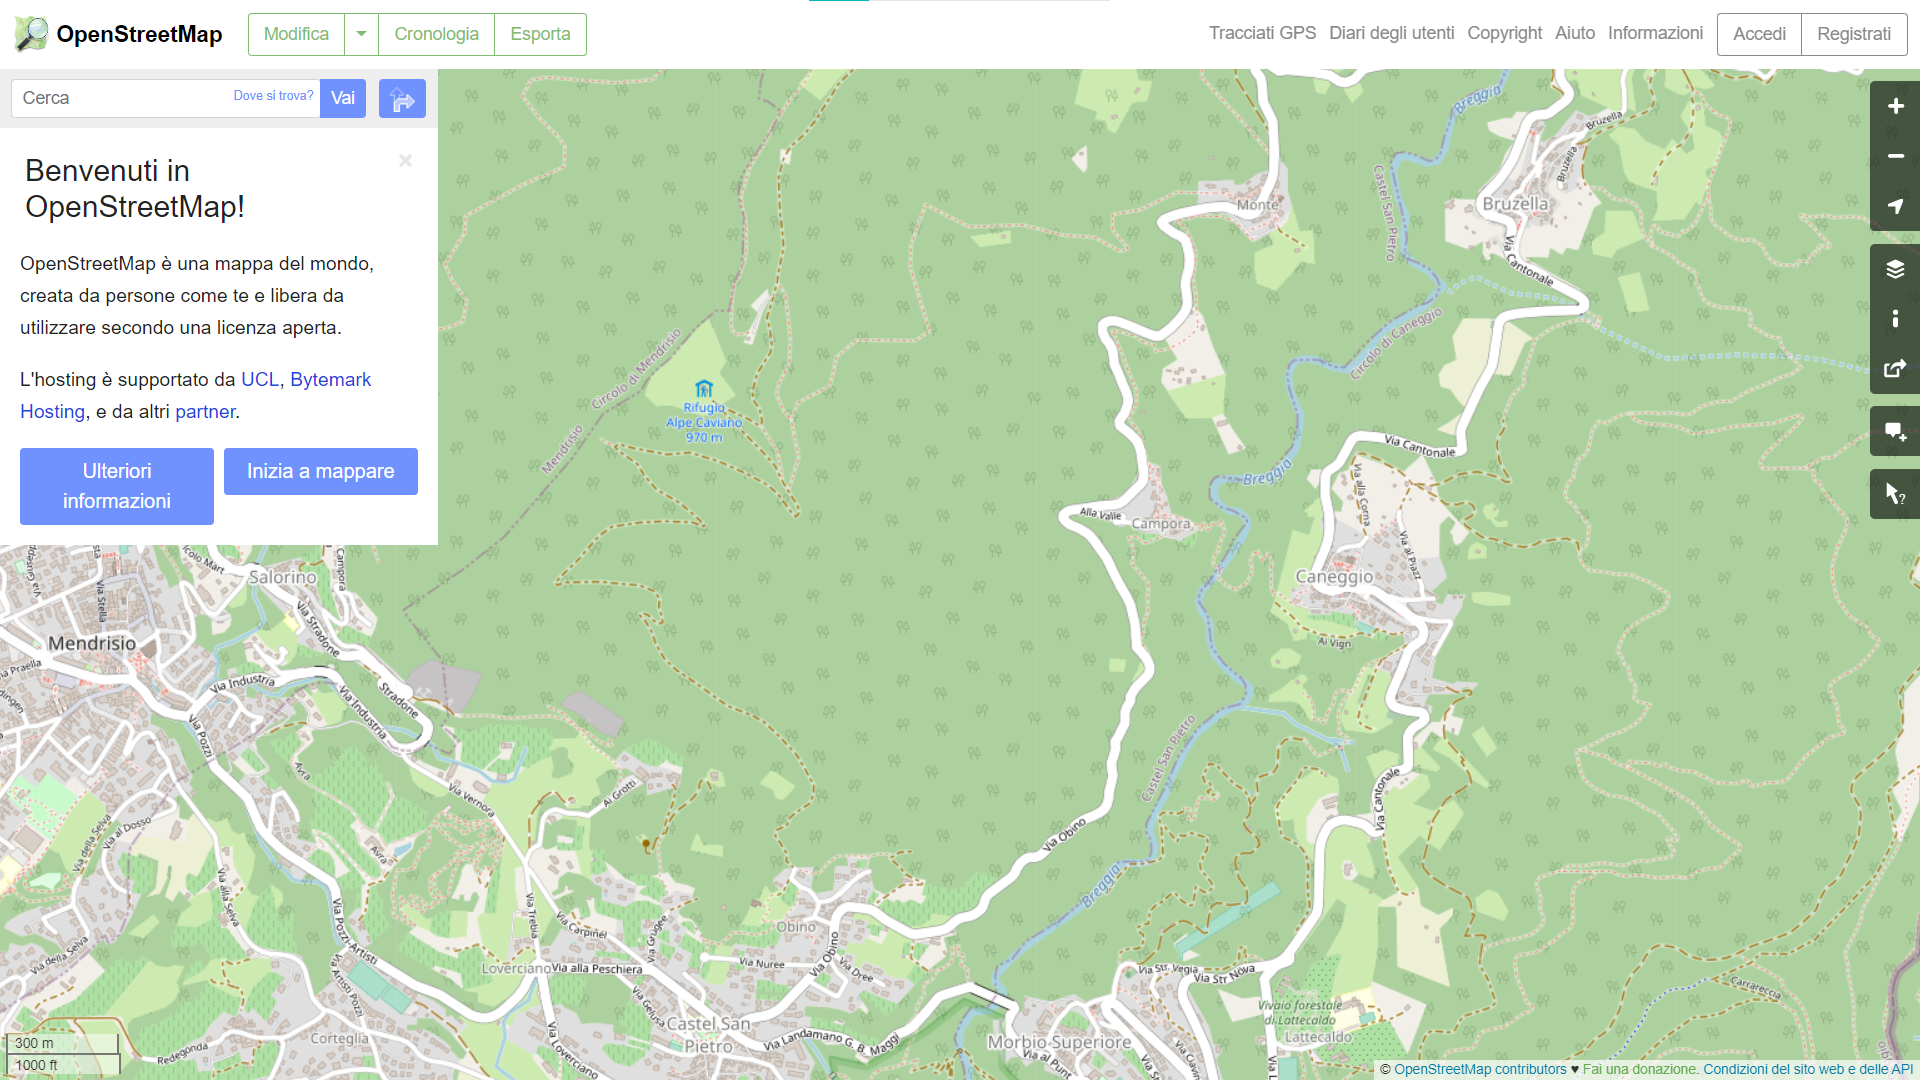
\includegraphics[width=1\textwidth]{Figures/OpenStreetMap.png}
    \caption{Selecting the area of interest in \textit{OpenStreetMap}}
      \label{fig:OpenStreetMap}
\end{figure}

Next, we have imported the \textit{.osm} file in MATLAB exploiting the \textit{Driving Scenario Designer} tool (Figure \ref{fig:DrivingScenarioTool}) provided as part of the Automated Driving Toolbox. The Driving Scenario Designer tool splits the whole selected route in as many pieces as the number of different streets names present. Then, the user can select only the pieces of road he/she is interested in and export its waypoints in a \textit{.mat} file.

\begin{figure}[H]
    \centering
    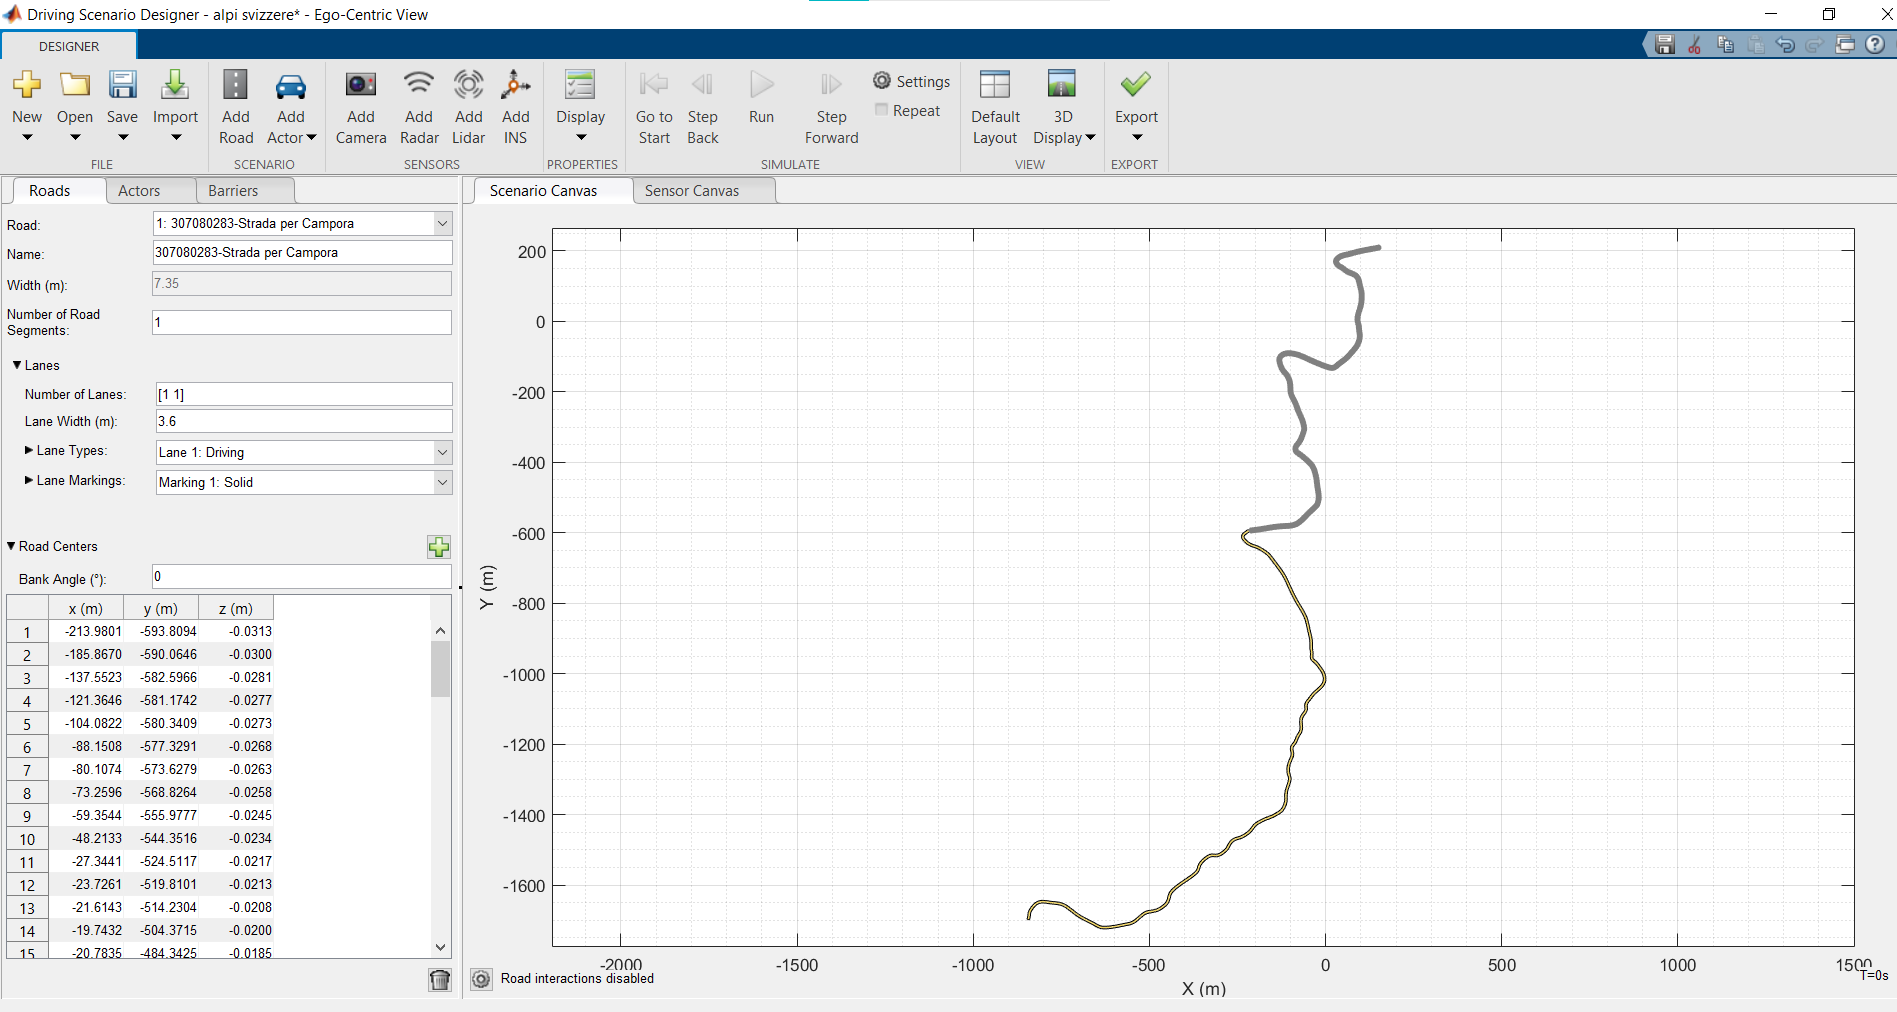
\includegraphics[width=1\textwidth]{Figures/DrivingScenarioTool.png}
    \caption{Importing maps on MATLAB using \textit{Driver Scenario Designer}}
      \label{fig:DrivingScenarioTool}
\end{figure}

Afterwards, the \textit{.mat} file is used to generate the corresponding map in the \textit{XY} reference frame.
Since the thus generated map is composed by an insufficient number of waypoints for our applications, we have decided to create a function \textit{ScenarioLoading} able to do an up-sample of the map because a higher density of points on it optimizes the path following algorithm. The up-sampling function interpolates linearly the original map with a fixed step depending on the reference speed and the sampling time selected for the controller. \\
It is worth mentioning, as shown in Figure \ref{fig:UpSample}, that the up-sampled path (in orange) and the original waypoints (in blue) slightly deviate in some sections of the route due to the smoothing applied in order to obtain a more gentle trajectory.

\begin{figure}[H]
    \centering
    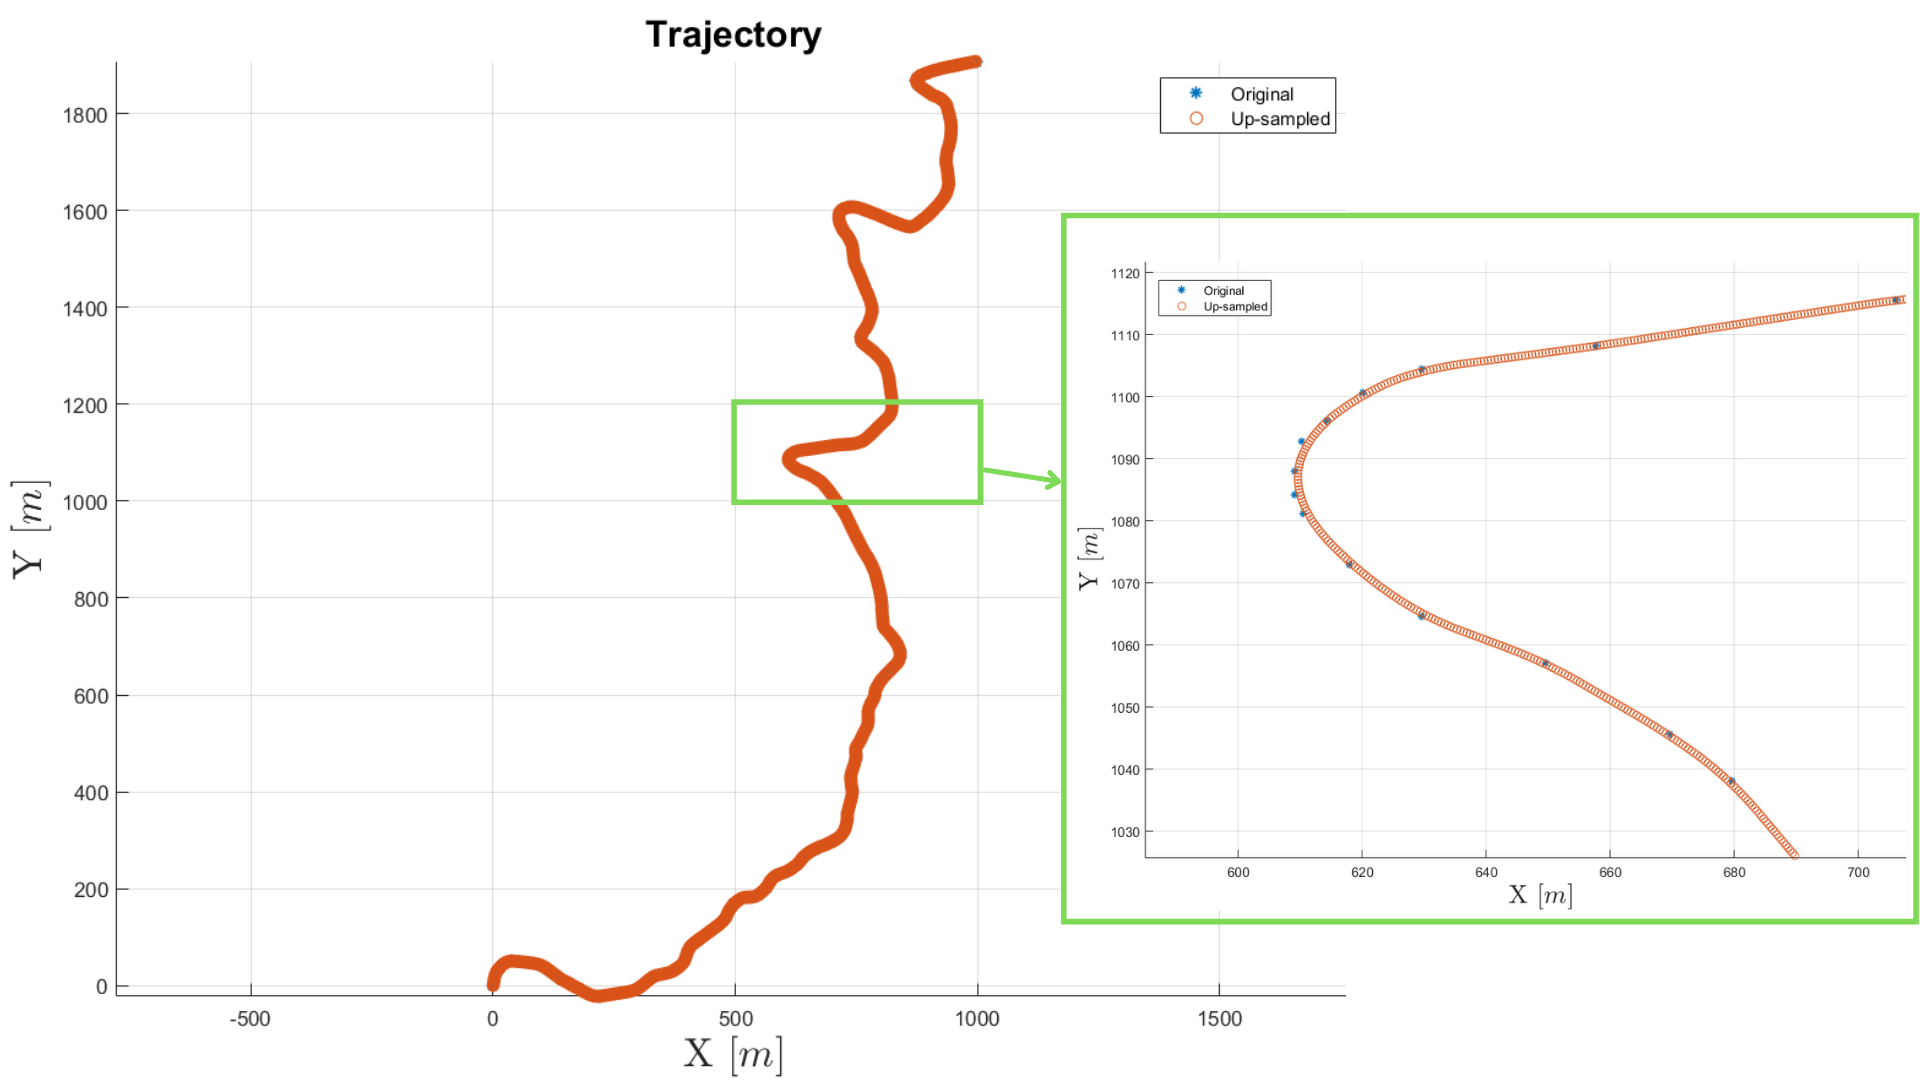
\includegraphics[width=1\textwidth]{Figures/UpSample.png}
    \caption{Comparison between original and up-sampled path}
      \label{fig:UpSample}
\end{figure}

%%%%%%%%%%%%%%%%%%%%%%%%%%%%%%%%%%%%%%%%%%%%%%%%

%\subsection{Obstacles acquisition}
\section{Constraints}
In this section we are going to introduce the constraints we have used for the project. A plausible set of constraints is fundamental in order to perform a realistic simulation, which is required in order to have reasonable simulation outcomes. 
\subsection{Actuators constraints}

The vehicle model presented in the Section \ref{chap:Vehicle_model} assumes that the inputs $\delta_f$ (front steering angle) and Throttle (driving and braking) can be controlled
directly. In practice, however, low-level controllers are used to transform the aforementioned
commands into physical control signals.
\subsubsection{Steering angle constraints}
Regarding the steering angle control, we suppose that our MPC directly affects the Electronic Power Steering (EPS) system by sending to it the target steering wheel position. Then, the EPS control unit calculates the optimal steering output based on the target steering wheel position received and sends the information to an electric motor to provide the necessary action on the wheels.
For the project, we have assumed this link to be ideal and so our MPC directly control the angle of our front wheels. The values used are reported in the Table \ref{tab:steering} and they have been chosen according to real data\cite{forkenbrock2005assessment}.

\begin{table}[H]
\begin{center}
\begin{tabular}{lllll}
\cline{2-3}
\multicolumn{1}{l|}{}                         & \multicolumn{1}{l|}{\textbf{min}} & \multicolumn{1}{l|}{\textbf{max}} &  &  \\ \cline{1-3}
\multicolumn{1}{|l|}{\textbf{Steering angle}} & \multicolumn{1}{l|}{-36 $deg$}      & \multicolumn{1}{l|}{36 $deg$}      &  &  \\ \cline{1-3}
\multicolumn{1}{|l|}{\textbf{Steering rate}}  & \multicolumn{1}{l|}{-60 $deg/s$}    & \multicolumn{1}{l|}{60 $deg/s$}    &  &  \\ \cline{1-3}
\end{tabular}
\caption{Steering constraints}
\label{tab:steering}

\end{center}
\end{table}

\subsubsection{Throttle constraints}
As stated in Section \ref{chap:Vehicle_model} the vehicle model used in our simulation is,  more or less, independent of the longitudinal dynamics of the vehicle. Moreover, the set of simulation we carry out are to be performed at constant speed, as close as possible to the target speed value. 
Physical limits on the actuators and comfort requirements impose bounds on the throttle and its rate of change according to the Table \ref{tab:throttle}.

\begin{table}[H]
\begin{center}
\begin{tabular}{lllll}
\cline{2-3}
\multicolumn{1}{l|}{} & \multicolumn{1}{l|}{\textbf{min}} & \multicolumn{1}{l|}{\textbf{max}} &  &  \\ \cline{1-3}
\multicolumn{1}{|l|}{\textbf{Throttle}} & \multicolumn{1}{l|}{-7.85 $m/s^2$}  & \multicolumn{1}{l|}{4 $m/s^2$} &  &  \\ \cline{1-3}
\multicolumn{1}{|l|}{\textbf{Throttle rate}} & \multicolumn{1}{l|}{-20 $m/s^3$}    & \multicolumn{1}{l|}{8 $m/s^3$} &  &  \\ \cline{1-3}
\end{tabular}
\caption{Throttle constraints}
\label{tab:throttle}
\end{center}
\end{table}

\subsection{Output/State constraints} Tbd
% - Output/State: Lane keeping and obstacle avoidance


%\include{Chapters/SafetyDistance}






\newpage
\bibliography{Compliance.bib}
\bibliographystyle{unsrt}

\end{document}  
